\chapter{進入保護模式} \label{CHpm}

前面我們看到,~通過一些很簡單的程式碼,~我們做到了啟動一個微型系統,~載入檔案系統中的檔案到記憶體並運行的功能。應該注意的是,~在前面的程式碼中我們使用的記憶體空間都很小。我們看一下~boot.bin~和~LOADER.BIN~的大小就能感覺出來(當然,~可執行檔案小未必使用記憶體空間小,~但是這兩個檔案也太小了~\smiley)。

\begin{Command}
$ ls -l boot.bin LOADER.BIN 
-rwxr-xr-x 1 solrex solrex 512 2008-04-26 16:34 boot.bin
-rwxr-xr-x 1 solrex solrex  15 2008-04-26 16:34 LOADER.BIN
\end{Command}

boot.bin~是~512~個~byte~(其中還有我們填充的內容,~實際指令只有~480~個~byte~),~而~LOADER.BIN~更過分,~只有~15~個~byte~大小。可想而知這兩個文件在記憶體中能使用多大的空間吧。如果讀者有些組合語言經驗的話,~就會發現我們在前面的程序中使用的存儲器尋址都是在真實模式下進行的,~即:由段暫存器(cs,~ds:~16-bit)配合段內偏移位址(16-bit)來定位一個實際的~20-bit~物理位址,~所以我們前面的程序最多支持~$2^{20} = 2^{10}*2^{10} = 1024*1024$ bytes = 1MB~的尋址空間。

哇,~~1MB~不小了,~我們的作業系統加一起連~1KB~都用不到,~~1MB~尋址空間足夠了。但是需要考慮到的一點是,~就拿我們現在用的~1.44MB的(已經被淘汰的)軟盤標準來說,~如果軟盤上某個文件超過~1MB~,~我們的作業系統就沒辦法處理了。那麼如果以後把作業系統安裝到硬盤上之後呢?我們就沒辦法處理稍微大一點的文件了。

所以我們要從最原始的~Intel 8086/8088 CPU~的真實模式中跳出來,~進入~Intel 80286~之後系列~CPU~給我們提供的保護模式。這還將為我們帶來其它更多的好處,~具體內容請繼續往下讀。

\section{真實模式和保護模式}

\BOXED{0.9\textwidth}{
\danger\\ 如果您需要更詳細的知識,~也許您更願意去讀 Intel 的手冊,~本節內容主要集中在:\href{http://download.intel.com/design/processor/manuals/253668.pdf}{Intel\textregistered~64 and IA-32 Architectures Software Developer's Manual, Volume 3A: System Programming Guide}, 第~2~章和第~3~章.\enddanger
}

\subsection{一段歷史}

Intel~公司在~1978~年發布了一款~16~位字長~CPU: 8086~,~最高頻率~5 MHz$\sim$10 MHz~,~集成了~29,000~個晶體管,~這款在今天感覺像玩具一樣的~CPU~卻是奠定今天~Intel PC~芯片市場地位的最重要的產品之一。雖然它的後繼者~8088~,~加強版的~8086~(增加了一個~8~比特的外部總線)才是事實上的~IBM~兼容機(PC,~個人電腦)雛形的核心,~但人們仍然習慣于用~8086~作為廠商標志代表~Intel~。

因為受到字長(16~位)的限制,~如果僅僅使用單個暫存器尋址,~~8086~僅僅能訪問~64KB($2^{16}$)~的位址空間,~這顯然不能滿足一般要求,~而當時~1MB($2^{20}$)~對于一般的應用就比較足夠了,~所以~8086~使用了~20~bit~的位址線。

在~8086~剛發布的時候,~沒有「真實模式」這個說法,~因為當時的~Intel CPU~只有一種模式。在~Intel~以後的發布中,~~80286~引入了“保護模式”尋址方式,~將~CPU~的尋址範圍擴大到~16($2^{24}$) MB~,~但是~80286~仍然是一款~16~位~CPU~,~這就限制了它的廣泛應用。但是“真實模式”這個說法,~就從~80286~開始了。

接下來的發展就更快了,~1985~年發布的~i386~首先讓~PC CPU~進入了~32~位時代,~由此而帶來的好處顯而易見,~尋址能力大大增強,~但是多任務處理和虛擬存儲器的需求仍然推動著~i386~向更完善的保護模式發展。下面我們來了解一下“真實模式”和“保護模式”的具體涵義。

\subsection{真實模式}

真實模式(real mode),~有時候也被成為真實位址模式(real address mode)或者兼容模式(compatibility mode)是~Intel 8086 CPU~以及以其為基礎發展起來的~x86~兼容~CPU~採用的一種操作模式。其主要的特點有:20~比特的分段訪問的記憶體位址空間(即~1~MB~的尋址能力);程序可直接訪問~BIOS~中斷和外設;硬件層不支持任何記憶體保護或者多任務處理。~80286~之後所有~x86 CPU~在加電自舉時都是首先進入真實模式;~80186~以及之前的~CPU~只有一種操作模式,~相當于真實模式。

\subsection{保護模式}

保護模式(protected mode),~有時候也被成為保護的虛擬位址模式(protected virtual address mode),~也是一種~x86~兼容~CPU~的工作模式。保護模式為系統軟件實現虛擬記憶體、分頁機制、安全的多任務處理的功能支持,~還有其它為作業系統提供的對應用程序的控制功能支持,~比如:權限、真實模式應用程序兼容、虛擬~8086~模式。

\subsection{真實模式和保護模式的尋址模式}

前面提到過,~真實模式下的位址線是~20~bit~的,~所以真實模式下的尋址模式使用分段方式來解決~16~位字長機器提供~20~bit~位址空間的問題。這個分段方法需要程序員在編制程序的過程中將存儲器劃分成段,~每個段內的位址空間是線性增長的,~最大可達~64K($2^16$),~
這樣段位址就可以使用~16~位表示。段基址(~20-bit~)的最低~4~位必須是~0~,~這樣段基址就可以使用~16~位段位址來表示,~需要時將段位址左移~4~位就得到段起始位址。除了便于尋址之外,~分段還有一個好處,~就是將程序的程式碼段、資料段和堆堆疊段等隔離開,~避免相互之間產生幹擾。

當計算某個單元的物理位址時,~比如組合語言中的一個~Label~,~就通過段位址(~16-bit~)左移~4~位得到段基址(~20-bit~),~再加上該單元(~Label~)的段偏移量(~16-bit~)來得到其物理位址(~20-bit~),~如圖~\ref{rm_addr}~所示。

\begin{figure*}[!t]
\centerline{\subfloat[真實模式尋址模型]{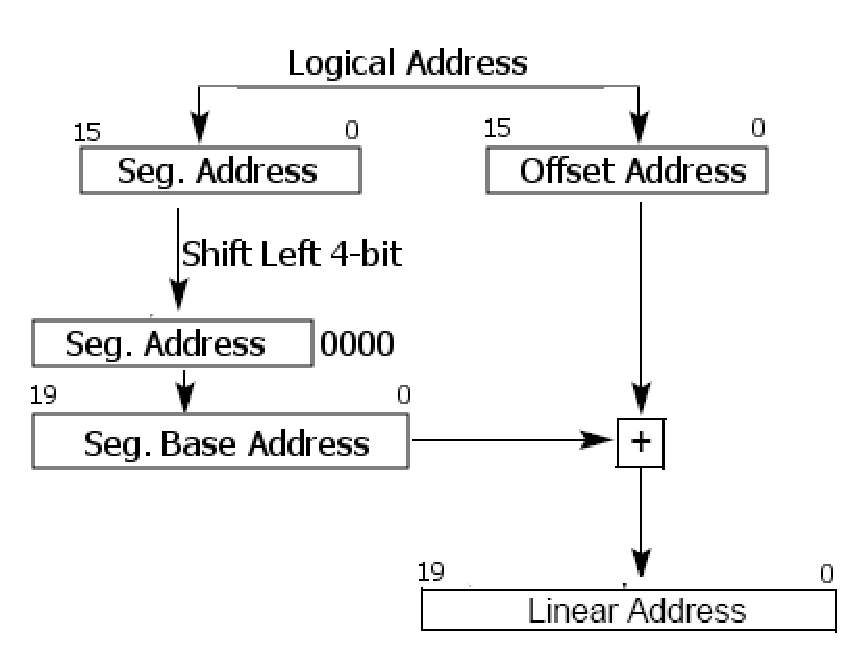
\includegraphics[width=.48\textwidth,keepaspectratio]{rm_addr}%
\label{rm_addr}}
\hfil
\subfloat[保護模式尋址模型]{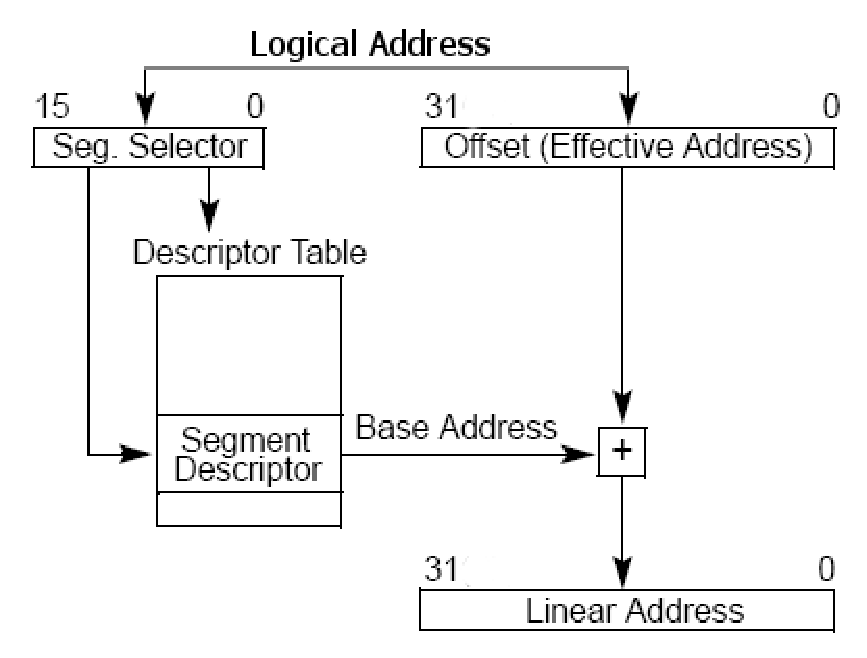
\includegraphics[width=.48\textwidth,keepaspectratio]{protected_seg}%
\label{protected_seg}}}
\caption{真實模式與保護模式尋址模型比較}
\label{real_vs_pro}
\end{figure*}

一般情況下,~段位址會被放在四個段暫存器中,~即:程式碼段~CS,~資料段~DS,~堆堆疊段~SS~和附加段~ES~暫存器。這樣在加載數據或者控制程序運行的時候,~只需要一個偏移量參數,~CPU~會自動用對應段的起始位址加上偏移量參數來得到需要的位址。(後繼~CPU~又加上了兩個段暫存器~FS~和~GS~,~不過使用方式是基本一樣的。)

由此可見,~真實模式的尋址模式是很簡單的,~就是用兩個~16~位邏輯位址(段位址:偏移位址)組合成一個~20~bit~物理位址,~而保護模式的尋址方式就要稍微復雜一點了。

\BOXED{0.9\textwidth}{
Intel~的~CPU~在保護模式下是可以選擇打開分頁機制的,~但為了簡單起見,~我們先不開啟分頁機制,~所以下面的講解針對只有分段機制的保護模式展開。
}

在保護模式下,~每個單元的物理位址仍然是由邏輯位址表示,~但是這個邏輯位址不再由(段位址:偏移位址)組成了,~而是由(段選擇子:偏移位址)表示。這裡的偏移位址也變成了~32~位的,~所以段空間也比真實模式下大得多。偏移位址的意思和真實模式下並沒有本質不同,~但段位址的計算就要復雜一些了,~如圖~\ref{protected_seg}~所示。段基址(Segment Base Address)被存放在段描述符(Segment Descriptor)中,~GDT(Global Descriptor Table,~全局段選擇子表)是保存著所有段選擇子的信息,~段選擇子(Segment Selector)是一個指向某個段選擇子的索引。

如圖~\ref{protected_seg}~所示,~當我們計算某個單元的物理位址時,~只需要給出(段選擇子:偏移位址),~CPU~會從~GDT~中按照段選擇子找到對應的段描述符,~從段描述符中找出段基址,~將段基址加上偏移量,~就得到了該單元的物理位址。

\section{與保護模式初次會面}

介紹完了保護模式和真實模式的不同,~下面我們就嘗試一下進入保護模式吧。在上一章我們已經實現了用啟動扇區加載引導文件,~所以這裡我們就不用再去管啟動扇區的事情了,~下面的修改均在~loader.S~中進行。上一章的~loader.S~僅僅實現在屏幕的上方中間打印了一個~\code{L}~,~下面我們的~loader.S~要進入保護模式來打印一些新東西。

首先,~我們來理清一下應該如何進入保護模式:

\begin{enumerate}
  \item 我們需要一個~GDT。由于保護模式的尋址方式是基于~GDT~的,~我們得自己寫一個~GDT~資料結構並將其載入到系統中。
  \item 我們需要為進入保護模式作準備。由于保護模式和真實模式運行方式不同,~在進入保護模式之前,~我們需要一些準備工作。
  \item 我們需要一段能在保護模式下運行的程式碼 demo,~以提示我們成功進入了保護模式。
\end{enumerate}

下面我們就來一步步完成我們的第一個保護模式~loader~。

\subsection{GDT~資料結構}

要寫~GDT,~首先得了解~GDT~的資料結構。GDT~實際上只是一個存儲段描述符的線性表(可以理解成一個段描述符數組),~對它的要求是其第一個段描述符置為空,~因為處理機不會去處理第一個段描述符,~所以理解~GDT~的資料結構難點主要在于理解段描述符的資料結構。

段描述符主要用來為處理機提供段位址,~段訪問控制和狀態信息。圖~\ref{seg_desc}~顯示了一個基本的段描述符結構:

\FIG{段描述符}{seg_desc}{.9\textwidth}

看到上面那麼多內容,~是不是感覺有點兒恐怖啊!其實簡單的來看,~我們現在最關注的是段基址,~就是圖~\ref{seg_desc}~中標記為~Base~的部分。可以看到,~段基址在段描述符中被分割為三段存儲,~分別是:Base 31:24, Base 23:16, Base Address 15:0,~把這三段拼起來,~我們就得到了一個~32~位的段基址。

有了段基址,~就需要有一個界限來避免程序跑丟發生段錯誤,~這個界限就是圖~\ref{seg_desc}~中標記為~Limit~的部分,~將~Seg. Limit 19:16~和~Segment Limit 15:0~拼起來我們就得到了一個~20~bit~的段界限,~這個界限就是應該是段需要的長度了。

下面還要說的就是那個~D/B Flag~,~D/B~代表~Default Operation Size~,~0~代表~16~位的段,~1~代表~32~位的段。為了充分利用~CPU~,~我們當然要設置為~32~位模式了。剩下那些亂七八糟的~Flag~呢,~無非就是提供段的屬性(程式碼段還是資料段?只讀還是讀寫?),~我們將在第~\ref{CHpm_desattr}~節為大家詳細介紹。

這些東西那麼亂,~難道要每次一點兒一點兒地計算嗎?放心,~程序員自有辦法,~請看下面的程序:

\VerbatimInput[fontfamily=tt,fontsize=\footnotesize,frame=lines, framerule=0.4mm, numbers=left, numbersep=3pt, tabsize=2, firstline=56, lastline=70]{../../src/chapter3/1/pm.h}
\codecaption{自動生成段描述符的宏定義(節自 chapter3/1/pm.h)}\label{CHpm_descm}

圖~\ref{CHpm_descm}~中所示,~就是自動生成段描述符的匯編宏定義。我們只需要給宏~Descriptor~三個參數:Base(段基址), Limit(段界限[段長度]), Attr(段屬性),~Descriptor~就會自動將三者展開放到段描述符中對應的位置。看看我們在程序中怎麼使用這個宏:

\VerbatimInput[fontfamily=tt,fontsize=\footnotesize,frame=lines, framerule=0.4mm, numbers=left, numbersep=3pt, tabsize=2, firstline=21, lastline=26]{../../src/chapter3/1/loader.S}
\codecaption{自動生成段描述符的宏使用示例(節自 chapter3/1/loader.S)}\label{CHpm_descmu}

圖~\ref{CHpm_descmu}~中,~就利用~Descriptor~宏生成了三個段描述符,~形成了一個~GDT。注意到沒有,~第一個段描述符是空的(參數全為~0)。這裡~LABEL\_DESC\_CODE32~的段基址為~0~是因為我們無法確定它的準確位置,~它將在運行期被填入。

有人可能會產生疑問,~段基址和段界限什麼意思我們都知道了,~那段屬性怎麼回事呢?~DA\_C, DA\_32, DA\_DRW~都是什麼東西啊?是這樣的,~為了避免手動一個一個置段描述符中的~Flag~,~我們預先定義了一些常用屬性,~用的時候只需要將這些屬性加起來作為宏~Descriptor~的參數,~就能將段描述符中的所有~flag~置上(記得~C~語言中~fopen~的參數嗎?)。這些屬性的定義如下(沒必要細看,~用的時候再找即可):

\VerbatimInput[fontfamily=tt,fontsize=\footnotesize,frame=lines, framerule=0.4mm, numbers=left, numbersep=3pt, tabsize=2, firstline=11, lastline=55]{../../src/chapter3/1/pm.h}
\codecaption{預先設置的段屬性(節自 chapter3/1/pm.h)}\label{CHpm_segattr}

\subsection{保護模式下的~demo}

為什麼把這節提前到第~\ref{CHpm_secloadgdt}~節前講呢?因為要寫入~GDT~正確的段描述符,~首先要知道段的信息,~我們就得先準備好這個段:

\VerbatimInput[fontfamily=tt,fontsize=\footnotesize,frame=lines, framerule=0.4mm, numbers=left, numbersep=3pt, tabsize=2, firstline=82, lastline=99]{../../src/chapter3/1/loader.S}
\codecaption{第一個在保護模式下運行的 demo(節自 chapter3/1/loader.S)}\label{CHpm_demo1}

其實這個段的作用很簡單,~通過操縱視頻段數據,~在屏幕中間打印一個紅色的"P"(和我們前面使用~BIOS~中斷來打印字符的方式有所不同)。

\subsection{加載~GDT} \label{CHpm_secloadgdt}

GDT~所需要的信息我們都知道了,~GDT~表也通過圖~\ref{CHpm_descmu}~中的程式碼實現了。那麼,~我們應該向~GDT~中填入缺少的信息,~然後載入~GDT~了。將~GDT~載入處理機是用~\code{lgdt}~匯編指令實現的,~但是~\code{lgdt}~指令需要存放~GDT~的基址和界限的指標作參數,~所以我們還需要知道~GDT~的位置和~GDT~的界限:

\VerbatimInput[fontfamily=tt,fontsize=\footnotesize,frame=lines, framerule=0.4mm, numbers=left, numbersep=3pt, tabsize=2, firstline=17, lastline=63]{../../src/chapter3/1/loader.S}
\codecaption{加載~GDT(節自 chapter3/1/loader.S)}\label{CHpm_loadgdt}

圖~\ref{CHpm_loadgdt}~中~\code{GdtPtr}~所指,~即為~GDT~的界限和基址所存放位置。某段描述符對應的~GDT~選擇子,~就是其段描述符相對于~GDT~基址的索引(在我們例子裡~GDT~基址為~\code{LABEL\_GDT}~指向的位置)。這裡需要注意的是,~雖然我們在程式碼中寫:

\begin{Command}
.set SelectorCode32, (LABEL_DESC_CODE32 - LABEL_GDT)
\end{Command}
但實際上段選擇子在使用時需要右移~3~個位作為索引去尋找其對應的段描述符,~段選擇子的右側~3~個位是為了標識~TI~和~RPL~的,~如圖~\ref{seg_selector}~所示,~這點我們將在第~\ref{CHpm_ldt}~節和第~\ref{CHpm_desattr}~節中詳細介紹。但是這裡為什麼能直接用位址相減得到段選擇子呢?因為段描述符的大小是~8~個~byte~,~用段描述符的位址相減的話,~位址差的最右側三個位就默認置~0~了。

在圖~\ref{CHpm_loadgdt}~中所示的程式碼,~主要幹了兩件事:第一,~將圖~\ref{CHpm_demo1}~所示~demo~的段基址放入~GDT~中對應的段描述符中;第二,~將~GDT~的基址放到~\code{GdtPtr}~所指的資料結構中,~並加載~\code{GdtPtr}~所指的資料結構到~GDTR~暫存器中(使用~\code{lgdt}~指令)。

\subsection{進入保護模式}

進入保護模式前,~我們需要將中斷關掉,~因為保護模式下中斷處理的機制和真實模式是不一樣的,~不關掉中斷可能帶來麻煩。使用~\code{cli}~匯編指令可以清除所有中斷~flag。

由于真實模式下僅有~20~條位址線:A0, A1, \ldots, A19,~所以當我們要進入保護模式時,~需要打開~A20~位址線。打開~A20~位址線有至少三種方法,~我們這裡採用~IBM~使用的方法,~通常被稱為:“Fast A20 Gate”,~即修改系統控制端口~92h~,~因為其端口的第~1~位控制著~A20~位址線,~所以我們只需要將~0b00000010~賦給端口~92h~即可。

當前面兩項工作完成後,~我們就可以進入保護模式了。方法很簡單,~將~cr0~暫存器的第~0~位~PE~位置為~1~即可使~CPU~切換到保護模式下運行。

\VerbatimInput[fontfamily=tt,fontsize=\footnotesize,frame=lines, framerule=0.4mm, numbers=left, numbersep=3pt, tabsize=2, firstline=64, lastline=77]{../../src/chapter3/1/loader.S}
\codecaption{進入保護模式(節自 chapter3/1/loader.S)}\label{CHpm_enablepm}

\subsection{特別的混合跳轉指令}

雖然已經進入了保護模式,~但由于我們的~CS~暫存器存放的仍然是真實模式下~16~位的段信息,~要跳轉到我們的~demo~程序並不是那麼簡單的事情。因為~demo~程序是~32~位的指令,~而我們現在仍然運行的是~16~位的指令。從~16~位的程式碼段中跳轉到~32~位的程式碼段,~不是一般的~near~或~far~跳轉指令能解決得了的,~所以這裡我們需要一個特別的跳轉指令。在這條指令運行之前,~所有的指令都是~16~位的,~在它運行之後,~就變成~32~位指令的世界。

在~Intel~的手冊中,~把這條混合跳轉指令稱為~far jump(ptr16:32)~,~在~NASM~手冊中,~將這條指令稱為~Mixed-Size Jump~,~我們就沿用~NASM~的說法,~將這條指令稱為混合字長跳轉指令。NASM~提供了這條指令的組合語言實做:
\begin{Command}
jmp dword 0x1234:0x56789ABC
\end{Command}
NASM~的手冊中說~GAS~沒有提供這條指令的實做,~我就用~.byte~偽程式碼直接寫了二進制指令:
\begin{Command}
/* Mixed-Size Jump. */
.2byte  0xea66
.4byte  0x00000000
.2byte  SelectorCode32
\end{Command}
但是有位朋友提醒我說現在的~GAS~已經支持混合字長跳轉指令(如圖~\ref{CHpm_mixedjmp}),~看來~NASM~的手冊好久沒有維護嘍~\smiley~。

\VerbatimInput[fontfamily=tt,fontsize=\footnotesize,frame=lines, framerule=0.4mm, numbers=left, numbersep=3pt, tabsize=2, firstline=77, lastline=82]{../../src/chapter3/1/loader.S}
\codecaption{混合字長跳轉指令(節自 chapter3/1/loader.S)}\label{CHpm_mixedjmp}

執行這條混合字長的跳轉指令時,~CPU~就會用段選擇子~\code{SelectorCode32}~去尋找~GDT~中對應的段,~由于段偏移是~0~,~所以~CPU~將跳轉到圖~\ref{CHpm_demo1}~中~demo~程序的開頭。為了方便閱讀,~整個~loader.S~的程式碼附在圖~\ref{CHpm_loader1}~中:

\VerbatimInput[fontfamily=tt,fontsize=\footnotesize,frame=lines, framerule=0.4mm, numbers=left, numbersep=3pt, tabsize=2, firstline=1, lastline=99]{../../src/chapter3/1/loader.S}
\codecaption{chapter3/1/loader.S}\label{CHpm_loader1}

\subsection{生成鏡像並測試}

使用與第~\ref{CHsmall_test}~節完全相同的方法,~我們可以將程式碼編譯並將~LOADER.BIN~拷貝到鏡像文件中。利用最新的鏡像文件啟動~VirtualBox~我們得到圖~\ref{vb_run_5}~。

可以看到,~屏幕的左側中央打出了一個紅色的~P~,~這就是我們那個在保護模式下運行的簡單~demo~所做的事情,~這說明我們的程式碼是正確的。從真實模式邁入保護模式,~這只是一小步,~但對于我們的作業系統來說,~這是一大步。從此我們不必再被限制到~20~bit~的位址空間中,~有了更大的自由度。

\FIG{第一次進入保護模式}{vb_run_5}{0.75\textwidth}

\section{段式存儲}

如果您仔細閱讀了圖~\ref{protected_seg}~,~您就會發現圖中並未提到~GDT~,~而是使用的~Descriptor Table(DT)~。這是因為對于~x86~架構的~CPU~來說,~~DT~總共有兩個:我們上節介紹過的~GDT~和下面要介紹的~LDT~。這兩個描述符表構成了~x86 CPU~段式存儲的基礎。顧名思義,~~GDT~作為全局的描述符表,~只能有一個,~而~LDT~作為局部描述符表,~就可以有很多個,~這也是以後作業系統給每個任務分配自己的存儲空間的基礎。

\subsection{LDT~資料結構} \label{CHpm_ldt}

\FIG{段選擇子資料結構}{seg_selector}{0.6\textwidth}

事實上,~~LDT~和~GDT~的差別非常小,~~LDT~段描述符的資料結構和圖~\ref{seg_desc}~所示是一樣的。所不同的就是,~~LDT~用指令~\code{lldt}~來加載,~並且指向~LDT~描述符項的段選擇子的~TI~位置必須標識為~1~,~如圖~\ref{seg_selector}~所示。這樣,~在使用~TI flag := 1~的段選擇子時,~作業系統才會從當前的~LDT~而不是~GDT~中去尋找對應的段描述符。

這裡值得注意的一點是:GDT~是由線性空間裡的位址定義的,~即~\code{lgdt}~指令的參數是一個線性空間的位址;而~LDT~是由~GDT~中的一個段描述符定義的,~即~\code{lldt}~指令的參數是~GDT~中的一個段選擇子。這是因為在加載~GDT~之前尋址模式是真實模式的,~而加載~GDT~後尋址模式變成保護模式尋址,~將~LDT~作為~GDT~中的段使用,~也方便作業系統在多個~LDT~之間切換。

\subsection{段描述符屬性} \label{CHpm_desattr}

我們在介紹圖~\ref{seg_desc}~時,~並沒有完全介紹段描述符的各個~Flag~和可能的屬性,~這一小節就用來專門介紹段描述符的屬性,~按照圖~\ref{seg_desc}~中的~Flag~從左向右的順序:

\begin{itemize}
\item{\textbf{G}}: G(Granularity,~粒度):如果~G flag~置為~0~,~段的大小以~byte~為單位,~段長度範圍是~\code{1 byte$\sim$1 MB}~;如果~G flag~置為~1~,~段的大小以~4 KB~為單位,~段長度範圍是~\code{4 KB $\sim$ 4 GB}~。
\item{\textbf{D/B}}:D/B(Default operation size/Default stack pionter size and/or upper Bound,~ 默認操作大小),~其意思取決于段描述符是程式碼段、資料段或者堆堆疊段。該~flag~置為~0~代表程式碼段/資料段為~16~位的;置為~1~代表該段是~32~位的。
\item{\textbf{L}}:L(Long, 長),~~L flag~是~IA-32e(Extended Memory 64 Technology)~模式下使用的標志。該~flag~置為~1~代表該段是正常的~64~位的程式碼段;置為~0~代表在兼容模式下運行的程式碼段。在~IA-32~架構下,~該位是保留位,~並且永遠被置為~0~。
\item{\textbf{AVL}}:保留給作業系統軟件使用的位。
\item{\textbf{P}}:P(segment-Present,~段佔用?) flag~用于標志段是否在記憶體中,~主要供記憶體管理軟件使用。如果~P flag~被置為~0~,~說明該段目前不在記憶體中,~該段指向的記憶體可以暫時被其它任務佔用;如果~P flag~被置為~1~,~說明該段在記憶體中。如果~P flag~為~0~的段被訪問,~處理機會產生一個~segment-not-present(\#NP)~異常。
\item{\textbf{DPL}}:DPL(Descriptor Privilege Level)域標志著段的權限,~取值範圍是從~0$\sim$3(2-bit)~,~0~代表著最高的權限。關于權限的作用,~我們將在下節討論。
\item{\textbf{S}}:S(descriptor type) flag~標志著該段是否系統段:置為~0~代表該段是系統段;置為~1~代表該段是程式碼段或者資料段。
\item{\textbf{Type}}:Type~域是段描述符裡最復雜的一個域,~而且它的意義對于程式碼/資料段描述符和系統段/門描述符是不同的,~下面我們用兩張表來展示當~Type~置為不同值時的意義。

表~\ref{code_data_types}~所示即為程式碼/資料段描述符的所有~Type~可能的值(0-15, 4-bit)以及對應的屬性含意,~表~\ref{sys_gate_types}~所示為系統段/門描述符的~Type~可能的值以及對應的屬性含意。這兩張表每個條目的內容是自明的,~而且我們在後面的討論中將不止一次會引用這兩張表的內容,~所以這裡對每個條目暫時不加詳細闡述。

\begin{center}\begin{longtable}{c|c|c|c|c|c|l}
\caption[]{程式碼/資料段描述符的~Type~屬性列表}\label{code_data_types}\\
\hline
\multicolumn{5}{c|}{\textbf{Type Field}} & \textbf{Descriptor Type} & \textbf{Description}\bigstrut\\
\cline{1-5}
\textbf{Decimal} & \textbf{11} & \textbf{10} & \textbf{9} & \textbf{8} & & \\
        &    &  \textbf{E} & \textbf{W} & \textbf{A} & & \\
\hline
0 & 0 & 0 & 0 & 0 & Data & Read-Only\\
1 & 0 & 0 & 0 & 1 & Data & Read-Only, Accessed\\
2 & 0 & 0 & 1 & 0 & Data & Read/Write\\
3 & 0 & 0 & 1 & 1 & Data & Read/Write, Accessed\\
4 & 0 & 1 & 0 & 0 & Data & Read-Only, Expand-down\\
5 & 0 & 1 & 0 & 1 & Data & Read-Only, Expand-down, Accessed\\
6 & 0 & 1 & 1 & 0 & Data & Read/Write, Expand-down\\
7 & 0 & 1 & 1 & 1 & Data & Read/Write, Expand-down, Accessed\\
\hline
        &    &  \textbf{C} & \textbf{R} & \textbf{A} & & \\
\hline
8 & 1 & 0 & 0 & 0 & Code & Execute-Only\\
9 & 1 & 0 & 0 & 1 & Code & Execute-Only, Accessed\\
10 & 1 & 0 & 1 & 0 & Code & Execute/Read\\
11 & 1 & 0 & 1 & 1 & Code & Execute/Read, Accessed\\
12 & 1 & 1 & 0 & 0 & Code & Execute-Only, Conforming\\
13 & 1 & 1 & 0 & 1 & Code & Execute-Only, Conforming, Accessed\\
14 & 1 & 1 & 1 & 0 & Code & Execute/Read-Only, Conforming\\
15 & 1 & 1 & 1 & 1 & Code & Execute/Read-Only, Conforming, Accessed\\
\hline
\end{longtable}\end{center}

\begin{center}\begin{longtable}{c|c|c|c|c|l}
\caption[]{系統段/門描述符的~Type~屬性列表}\label{sys_gate_types}\\
\hline
\multicolumn{5}{c|}{\textbf{Type Field}} & \textbf{Description}\bigstrut\\
\hline
\textbf{Decimal} & \textbf{11} & \textbf{10} & \textbf{9} & \textbf{8} & \textbf{32-Bit Mode}\\
\hline
0 & 0 & 0 & 0 & 0 & Reserved\\
1 & 0 & 0 & 0 & 1 & 16-bit TSS(Available)\\
2 & 0 & 0 & 1 & 0 & LDT\\
3 & 0 & 0 & 1 & 1 & 16-bit TSS(Busy)\\
4 & 0 & 1 & 0 & 0 & 16-bit Call Gate\\
5 & 0 & 1 & 0 & 1 & Task Gate\\
6 & 0 & 1 & 1 & 0 & 16-bit Interrupt Gate\\
7 & 0 & 1 & 1 & 1 & 16-bit Trap Gate\\
8 & 1 & 0 & 0 & 0 & Reserved\\
9 & 1 & 0 & 0 & 1 & 32-bit TSS(Available)\\
10 & 1 & 0 & 1 & 0 & Reserved\\
11 & 1 & 0 & 1 & 1 & 32-bit TSS(Busy)\\
12 & 1 & 1 & 0 & 0 & 32-bit Call Gate\\
13 & 1 & 1 & 0 & 1 & Reserved\\
14 & 1 & 1 & 1 & 0 & 32-bit Interrupt Gate\\
15 & 1 & 1 & 1 & 1 & 32-bit Trap Gate\\
\hline
\end{longtable}\end{center}

\end{itemize}

\subsection{使用~LDT~}

從目前的需求來看,~對~LDT~並沒有非介紹不可的理由,~但是理解~LDT~的使用,~對理解段式存儲和處理機多任務存儲空間分配有很大的幫助。所以我們在下面的程式碼中實現幾個簡單的例子:一,~建立~32~位數據和堆堆疊兩個段並將描述符添加到~GDT~中;二,~添加一段簡單程式碼,~並以其段描述符為基礎建立一個~LDT;三,~在~GDT~中添加~LDT~的段描述符並初始化所有~DT~;四,~進入保護模式下運行的~32~位程式碼段後,~加載~LDT~並跳轉執行~LDT~中包含的程式碼段。

首先,~建立~32~位全局資料段和堆堆疊段,~並將其描述符添加到~GDT~中:

\VerbatimInput[fontfamily=tt,fontsize=\footnotesize,frame=topline, framerule=0.4mm, numbers=left, numbersep=3pt, tabsize=2, firstline=50, lastline=62]{../../src/chapter3/2/loader.S}
\VerbatimInput[fontfamily=tt,fontsize=\footnotesize,frame=bottomline, framerule=0.4mm, numbers=left, numbersep=3pt, tabsize=2, firstline=22, lastline=41]{../../src/chapter3/2/loader.S}
\codecaption{32~位全局資料段和堆堆疊段,~以及對應的~GDT~結構(節自 chapter3/2/loader.S)}\label{CHpm_add_ds}

在圖~\ref{CHpm_add_ds}~中,~我們首先建立了一個全局的資料段,~並在資料段裡放置了兩個字符串,~分別用來進入保護模式後和跳轉到~LDT~指向的程式碼段後作為信息輸出。然後又建立了一個全局的堆堆疊段,~為堆堆疊段預留了~512~~byte~的空間,~並將堆疊頂設置為距堆疊底~511~~byte~處。然後與上節介紹的類似,~將資料段和堆堆疊段的段描述符添加到~GDT~中,~並設置好對應的段選擇子。

要注意到資料段、堆堆疊段和程式碼段的段描述符屬性不盡相同。資料段的段描述符屬性是~\code{DA\_DRW}~,~回憶我們前面~pm.h~的內容(圖~\ref{CHpm_segattr}~),~~\code{DA\_DRW}~的內容是~\code{0x92},~用二進制就是~\code{10010010},~其後四位就對應著圖~\ref{code_data_types}~中的第二~2(0010)~項,~說明這個段是可讀寫的資料段;前四位對應著~\code{P|DPL|S}~三個~flag~,~即~\code{P:1, DPL:00, S:1}~,~與第~\ref{CHpm_desattr}~節結合理解,~意思就是該段在記憶體中,~為最高的權限,~非系統段。所以我們可以看到~pm.h~中的各個屬性變量定義,~就是將二進制的屬性值用可理解的變量名表示出來,~在用的時候直接加上變量即可。

同理我們也可以分別來理解~GDT~中堆堆疊段和程式碼段描述符的屬性定義。因為不同類型的屬性使用的是段描述符中不同的位,~所以不同類型的屬性可以直接相加得到復合的屬性值,~例如堆堆疊段的~\code{(DA\_DRWA + DA\_32)}~,~其意思類似于~\code{C++}~中~\code{fstream}~打開文件時可以對模式進行算術或(\code{ios\_base::in | ios\_base::out})來得到復合參數。

其次,~添加一段簡單的程式碼,~並以其描述符為基礎建立一個~LDT:

\VerbatimInput[fontfamily=tt,fontsize=\footnotesize,frame=topline, framerule=0.4mm, numbers=left, numbersep=3pt, tabsize=2, firstline=114, lastline=140]{../../src/chapter3/2/loader.S}
\VerbatimInput[fontfamily=tt,fontsize=\footnotesize,frame=bottomline, framerule=0.4mm, numbers=left, numbersep=3pt, tabsize=2, firstline=42, lastline=49]{../../src/chapter3/2/loader.S}
\codecaption{32~位程式碼段,~以及對應的~LDT~結構(節自 chapter3/2/loader.S)}\label{CHpm_build_ldt}

\code{LABEL\_CODEA}~就是我們為~LDT~建立的簡單程式碼段,~其作用就是操作顯存在屏幕的第~12~行開始用紅色的字打印出偏移~\code{OffsetLDTMessage}~指向的全局資料段中的字符串。下面就是以~\code{LABEL\_CODEA}~為基礎建立的~LDT~,~從~LDT~的結構來說,~與~GDT~沒有區別,~但是我們不用像~\code{GdtPtr}~再建立一個~\code{LdtPtr}~,~因為~LDT~實際上是在~GDT~中定義的一個段,~不用真實模式的線性位址表示。

LDT~的選擇子是與~GDT~選擇子有明顯區別的,~圖~\ref{seg_selector}~清楚地解釋了這一點,~所以指向~LDT~的選擇子都應該將~TI~位置~1~,~在圖~\ref{CHpm_build_ldt}~的最後一行也實現了這一操作。

第三,~在~GDT~中添加~LDT~的段描述符(在圖~\ref{CHpm_add_ds}~中我們已經能看到在~GDT~中添加好了~LDT~的段描述符),~初始化所有段描述符。由于初始化段描述符屬于重復性工作,~我們在~pm.h~中添加一個匯編宏~\code{InitDesc}~來幫我們做這件事情。

\VerbatimInput[fontfamily=tt,fontsize=\footnotesize,frame=lines, framerule=0.4mm, numbers=left, numbersep=3pt, tabsize=2, firstline=84, lastline=96]{../../src/chapter3/2/pm.h}
\codecaption{自動初始化段描述符的宏程式碼(節自 chapter3/2/pm.h)}\label{CHpm_initdesc}

\VerbatimInput[fontfamily=tt,fontsize=\footnotesize,frame=lines, framerule=0.4mm, numbers=left, numbersep=3pt, tabsize=2, firstline=63, lastline=112]{../../src/chapter3/2/loader.S}
\codecaption{在真實模式程式碼段中初始化所有段描述符(節自 chapter3/2/loader.S)}\label{CHpm_init_dts}

初始化各個段描述符的方式與上一節介紹的初始化~GDT~描述符的方式沒有什麼本質不同,~因為屬性都已經預設好,~運行時只需要將段位址填入描述符中的位址域即可,~程式碼都是重復的。我們引入宏~\code{InitDesc}的幫助,~能大大縮短程式碼長度,~增強程式碼的可讀性。

第四,~進入保護模式下運行的~32~位程式碼段後,~加載~LDT~並跳轉執行~LDT~中包含的程式碼段:

\VerbatimInput[fontfamily=tt,fontsize=\footnotesize,frame=lines, framerule=0.4mm, numbers=left, numbersep=3pt, tabsize=2, firstline=141, lastline=176]{../../src/chapter3/2/loader.S}
\codecaption{在保護模式程式碼段中加載~LDT~並跳轉執行~LDT~程式碼段(節自 chapter3/2/loader.S)}\label{CHpm_run_ldt}

在~\code{LABEL\_SEG\_CODE32}~中前幾行,~我們可以看到非常熟悉的匯編指令,~和一般匯編程序開頭初始化數據/程式碼/堆堆疊段暫存器的指令非常像,~只不過這裡賦給幾個暫存器的參數都是段選擇子,~而不是一般的位址。該程式碼段剩下的內容和前面圖~\ref{CHpm_build_ldt}~中~\code{LABEL\_CODEA}~一樣,~都是打印一個字符串,~只不過這裡選擇在第~10~行(屏幕左側中央)打印。

為了方便閱讀,~整個~loader.S~的程式碼附在圖~\ref{CHpm_loader2}~中。

\VerbatimInput[fontfamily=tt,fontsize=\footnotesize,frame=lines, framerule=0.4mm, numbers=left, numbersep=3pt, tabsize=2]{../../src/chapter3/2/loader.S}
\codecaption{chapter3/2/loader.S}\label{CHpm_loader2}

\subsection{生成鏡像並測試}

使用與第~\ref{CHsmall_test}~節完全相同的方法,~我們可以將程式碼編譯並將~LOADER.BIN~拷貝到鏡像文件中。利用最新的鏡像文件啟動~VirtualBox~我們得到圖~\ref{vb_run_6}~。

\FIG{第一次進入保護模式}{vb_run_6}{0.75\textwidth}

可以看到,~該程序首先在屏幕左側中央(第~10~行)打印出來~\code{"Welcome to protect mode!\^{}-\^{}"}~,~這是由~GDT~中的~32~位程式碼段~\code{LABEL\_SEG\_CODE32}~打印出來的,~標志著我們成功進入保護模式;然後在屏幕的第~12~行打印出來~\code{"Aha, you jumped into a LDT segment."}~,~這個是由~LDT~中的~32~位程式碼段~\code{LABEL\_CODEA}~打印出來的,~標志著~LDT~的使用正確。因為這兩個字符串都是被存儲在~32~位全局資料段中,~這兩個字符串的成功打印也說明在~GDT~中添加的資料段使用正確。

\subsection{段式存儲總結}

段式存儲和頁式存儲都是最流行的計算機記憶體保護方式。段式存儲的含義簡單來說就是先將記憶體分為各個段,~然後再分配給程序供不同用途使用,~並保證對各個段的訪問互不幹擾。x86~主要使用段暫存器(得到的段基址)~\code{+}~偏移量來訪問段中數據,~也簡化了尋址過程。

在~x86~的初期真實模式下就使用著非常簡單的段式存儲方式,~如圖~\ref{rm_addr}~所示,~這種模式下分段主要是為了方便尋址和隔離,~沒有提供其它的保護機制。x86~保護模式下採用了更高級的段式存儲方式:用全局和局部描述符表存儲段描述符信息,~使用段選擇子表示各個段描述符,~如圖~\ref{protected_seg}~所示。

由于保護模式使用段描述符來保存段信息而不是像真實模式一樣直接使用段位址,~在段描述符中就可以添加一些屬性來限制對段的訪問權限,~如我們在第~\ref{CHpm_desattr}~節中討論的那樣。這樣,~通過在訪問段時檢查權限和屬性,~就能做到對程序段的更完善保護和更好的記憶體管理。

x86~使用全局描述符表(GDT)和局部描述符表(LDT)來實現不同需求下對程序段的控制,~作業系統使用唯一的一個~GDT~來維護一些和系統密切相關的段描述符信息,~為不同的任務使用不同的~LDT~來實現對多任務記憶體管理的支持,~簡化了任務切換引起的記憶體切換的難度。

\section{權限}

\BOXED{0.9\textwidth}{
\danger\\ 如果您需要更詳細的知識,~也許您更願意去讀 Intel 的手冊,~本節內容主要集中在:\href{http://download.intel.com/design/processor/manuals/253668.pdf}{Intel\textregistered~64 and IA-32 Architectures Software Developer's Manual, Volume 3A: System Programming Guide}, 第~4~章.\enddanger
}

權限是為了保護處理機資源而引入的概念。將同一個處理機上執行的不同任務賦予不同的權限,~可以控制該任務可以訪問的資源,~比如記憶體位址範圍、輸入輸出端口、和一些特殊指令的使用。在~x86~體系結構中,~共有~4~個權限別,~0~代表最高權限,~3~代表最低權限。由于在~x86~體系結構中,~n~級可以訪問的資源均可以被~0~到~n~級訪問,~這個模式被稱作~ring~模式,~相應地我們也將~x86~的對應權限稱作~ring n。

現代的~PC~作業系統的核心一般工作在~ring 0~下,~擁有最高的權限,~應用程序一般工作在~ring 3~下,~擁有最低的權限。雖然~x86~體系結構提供了~4~個權限,~但作業系統並不需要全部使用到這~4~個級別,~可以根據需要來選擇使用幾個權限。比如~Linux/Unix~和~Windows NT~,~都是只使用了~0~級和~3~級,~分別用于核心模式和用戶模式;而~DOS~則只使用了~0~級。

為了實施對程式碼段和資料段的權限檢驗,~x86~處理機引入了以下三種權限類型(請注意這裡提到的權限高低均為實際高低,~而非數值意義上的高低):

\begin{itemize}
\item{\textbf{CPL(Current Privilege Level)}}:當前權限,~存儲在~CS~和~SS~的~0, 1~位。它代表當前執行程序或任務的權限,~通常情況下與當前執行指令所在程式碼段的~DPL~相同。當程序跳轉到不同權限的程式碼段時,~CPL~會隨之修改。當訪問一致程式碼段(Conforming Code Segment)時,~對~CPL~的處理有些不同。一致程式碼段可以被不高于(數值上大于等于)該段~DPL~的權限程式碼訪問,~但是,~CPL~在訪問一致程式碼段時不會跟隨~DPL~的變化而更改。

\item{\textbf{DPL(Descriptor Privilege Level)}}:描述符權限,~定義于段描述符或門描述符中的~DPL~域(見圖~\ref{seg_desc}),~它限制了可以訪問此段資源的權限別。根據被訪問的段或者門的不同,~DPL~的意義也不同:
  \begin{itemize}
  \item{\textbf{資料段}}:資料段的~DPL~限制了可以訪問該資料段的最低權限。假如資料段的~DPL~為~1,~那麼只有~CPL~為~0,1~的程序才能訪問該資料段。
  \item{\textbf{非一致程式碼段(不使用~call gate~)}}:非一致程式碼段就是一般的程式碼段,~它的~DPL~表示可以訪問該段的權限,~程序或者任務的權限必須與該段的~DPL~完全相同才可以訪問該段。
  \item{\textbf{~call gate~}}:~call gate~的~DPL~限制了可以訪問該門的最低權限,~與資料段~DPL~的意思一樣。
  \item{\textbf{一致程式碼段和使用~call gate~訪問的非一致程式碼段}}:這種程式碼段的~DPL~表示可以訪問該段的最高權限。假如一致程式碼段的~DPL~是~2,~那麼~CPL~為~0,1~的程序就無法訪問該段。
  \item{\textbf{TSS(Task State Segment)}}:任務狀態段的~DPL~表示可以訪問該段的最低權限,~與資料段~DPL~的意思一樣。
  \end{itemize}

\item{\textbf{RPL(Requested Privilege Level)}}:請求權限,~定義于段選擇子的~RPL~域中(見圖~\ref{seg_selector})。它限制了這個選擇子可訪問資源的最高權限。比如一個段選擇子的~RPL~為~2~,~那麼使用這個段選擇子只能訪問~DPL~為~2~或者~3~的段,~即使使用這個段選擇子的程序當前權限(CPL)為~0~。就是說,~$\max{(CPL, RPL)}\le DPL$~才被允許訪問該段,~即當~CPL~小于~RPL~時,~RPL~起決定性作用,~反之亦然。使用~RPL~可以避免權限高的程序代替應用程序訪問該應用程序無權訪問的段。比如在系統呼叫時,~應用程序呼叫系統過程,~雖然系統過程的權限高($CPL=0$),~但是被呼叫的系統過程仍然無法訪問權限高于應用程序的段($DPL<RPL=3$),~就避免了可能出現的安全問題。
\end{itemize}

在將段描述符對應的段選擇子加載到段暫存器時,~處理機通過將~CPL, 段選擇子的~RPL~和該段的~DPL~相比較,~來判斷程序是否有權訪問另外一個段。如果~$CPL>\max{(RPL, DPL)}~$,~或者$\max{(CPL, RPL)}>DPL$,~那麼該訪問就是不合法的,~處理機就會產生一個常規保護異常(\texttt{\#}GP, General Protection Exception)。

\subsection{不合法的訪問請求示例}

我們來看一個不合法的訪問請求的例子,~在上一節的~loader.S~中把~\code{LABEL\_DESC\_DATA}~對應的描述符的~\code{DPL}~設置為~1,~然後將該資料段對應的段選擇子的~RPL~設置為~3,~即修改以下兩行:
\begin{Command}
LABEL_DESC_DATA:    Descriptor        0,      (DataLen - 1), (DA_DRW + DA_DPL1)
.set    SelectorData,   (LABEL_DESC_DATA   - LABEL_GDT + SA_RPL3)
\end{Command}

\FIGFIX{虛擬機出現異常,~黑屏}{vb_run_7}{0.75\textwidth}

\FIGFIX{虛擬退出後~VBox~主窗口顯示~Abort}{vb_main_4}{0.75\textwidth}

再~\code{make, sudo make copy},~用~VirtualBox~加載生成的鏡像運行一下,~就會發現虛擬機黑屏一會兒就會退出(如圖~\ref{vb_run_7}),~然後~VirtualBox~主窗口中顯示該虛擬機~Aborted(如圖~\ref{vb_main_4})。這是因為我們違反權限的規則,~使用~RPL=3~的選擇子去訪問~DPL=1~的段,~這個不合法的訪問請求引起處理機產生常規保護異常(\texttt{\#}GP)。而我們又沒有準備對應的異常處理模塊,~當處理機找不到異常處理程序時就只好退出了。


\subsection{控制權轉移的權限檢查}

在將控制權從一個程式碼段轉移到另一個程式碼段之前,~目標程式碼段的段選擇子必須被加載到~CS~中。處理器在這個過程中會查看目標程式碼段的段描述符以及對其界限、類型(見圖~\ref{seg_desc})和權限進行檢查。如果沒有錯誤發生,~CS~暫存器會被加載,~程序控制權被轉移到新的程式碼段,~從~EIP~指示的位置開始運行。

JMP, CALL, RET, SYSENTER, SYSEXIT, INT n~和~IRET~這些指令,~以及中斷和異常機制都會引起程序控制權的轉移。

JMP~和~CALL~指令可以實現以下~4~種形式的轉移:

\begin{itemize}
\item 目標操作數包含目標程式碼段的段選擇子。
\item 目標操作數指向一個包含目標程式碼段段選擇子的~call gate~描述符。
\item 目標操作數指向一個包含目標程式碼段段選擇子的任務狀態段。
\item 目標操作數指向一個任務門,~這個任務門指向一個包含目標程式碼段段選擇子的任務狀態段。
\end{itemize}

下面兩個小節將描述前兩種轉移的實現方法,~後兩種控制權轉移方法我們將在用到時再進行解釋。

\subsubsection{用~JMP~或~CALL~直接轉移}

用~JMP, CALL~和~RET~指令在段內進行近跳轉並沒有權限的變化,~所以對這類轉移是不進行權限檢查的;用~JMP, CALL~和~RET~在段間進行遠跳轉涉及到其它程式碼段,~所以要進行權限檢查。

對不通過~call gate~的直接轉移來說,~又分為兩種情形:

\begin{itemize}
\item{訪問非一致程式碼段}:當目標是非一致程式碼段時(目標段段描述符的~C flag~為~0~,~見圖~\ref{code_data_types}),~權限檢查要求呼叫者的~CPL~與目標程式碼段的~DPL~相等,~而且呼叫者使用的目標程式碼段段選擇子的~RPL~必須小于等于目標程式碼段的~DPL。我們之前的程式碼都屬于這種情形,~其中~$CPL=DPL=RPL=0$。
\item{訪問一致程式碼段}:當目標是一致程式碼段時(目標段段描述符的~C flag~為~1~,~見圖~\ref{code_data_types}),~權限檢查要求~$CPL \ge DPL$,~RPL~不被檢查,~而且轉移時並不修改~CPL。
\end{itemize}

總的來說,~通過~JMP~和~CALL~實行的都是一般的轉移,~最多從低權限轉移到高權限的一致程式碼段,~CPL~總是不變的。

\subsection{使用~call gate~轉移}\label{CHpm_callgate}

~call gate~是~x86~體系結構下用來控制程序在不同權限間轉移的一種機制。它的目的是使低權限的程式碼能夠呼叫高權限的程式碼,~這一機制在使用了記憶體保護和權限機制的現代作業系統中非常有用,~因為它允許應用程序在作業系統控制下安全地呼叫核心例程或者系統接口。

\FIG{~call gate~描述符}{callgate_desc}{.9\textwidth}

門其實也是一種描述符,~和段描述符類似。~call gate~描述符的資料結構如圖~\ref{callgate_desc}~所示。其實看起來這個~call gate~描述符的資料結構要比段描述符簡單一些,~至少從它的屬性來說,~沒有段描述符多。我們仍然只關注最重要的部分:首先是段選擇子(Segment Selector),~指定了通過這個~call gate~訪問的程式碼段;其次是段偏移量(Offset in Segment),~指定了要訪問程式碼段中的某個入口偏移;描述符權限(DPL),~代表此門描述符的權限;P,~代表此~call gate~是否可用;參數計數(Param. Count)記錄了如果發生堆疊切換的話,~有多少個選項參數會在堆疊間拷貝。

簡單來說,~~call gate~描述了由一個段選擇子和一個偏移所指定的目標程式碼段中的一個位址,~程序通過~call gate~將轉移到這個位址。下面我們通過一個簡單的例子來介紹一下~call gate~的基本使用方法。

\subsubsection{簡單的~call gate~轉移舉例}

為了使用~call gate~,~我們首先要給出一個目標段,~然後用該目標段的信息初始化~call gate~的門描述符,~最後用~call gate~的門選擇子實現門呼叫。

添加一個目標段我們已經做過很多次,~非常簡單。首先在上一節~loader.S~最後添加一個打印一個字符的程式碼段~\code{LABEL\_SEG\_CODECG},~接著將該段的段描述符~\code{LABEL\_DESC\_CODECG}~添加到~GDT~中,~然後為該段準備一個段選擇子~\code{SelectorCodeCG},~最後加入初始化該段描述符的程式碼:

\VerbatimInput[fontfamily=tt,fontsize=\footnotesize,frame=topline, framerule=0.4mm, numbers=left, numbersep=3pt, tabsize=2, firstline=197, lastline=211]{../../src/chapter3/3/loader.S}
\VerbatimInput[fontfamily=tt,fontsize=\footnotesize,frame=none, framerule=0.4mm, numbers=left, numbersep=3pt, tabsize=2, firstline=28, lastline=29]{../../src/chapter3/3/loader.S}
\VerbatimInput[fontfamily=tt,fontsize=\footnotesize,frame=none, framerule=0.4mm, numbers=left, numbersep=3pt, tabsize=2, firstline=43, lastline=44]{../../src/chapter3/3/loader.S}
\VerbatimInput[fontfamily=tt,fontsize=\footnotesize,frame=bottomline, framerule=0.4mm, numbers=left, numbersep=3pt, tabsize=2, firstline=92, lastline=94]{../../src/chapter3/3/loader.S}
\codecaption{添加~call gate~的目標段(節自 chapter3/3/loader.S)}\label{CHpm_codecg}

總的來看,~~\code{LABEL\_SEG\_CODECG}~指向的這個段和我們以前為了打印程序運行結果所使用的段沒有本質不同,~為了簡單起見,~這裡我們僅僅讓它打印一個字符~\code{'C'}~就返回。

用目標程式碼段~\code{LABEL\_SEG\_CODECG}~的信息初始化~call gate~的門描述符~\code{LABEL\_CG\_TEST},~以及門選擇子~\code{SelectorCGTest}。與匯編宏~\code{Descriptor}~類似,~我們這裡使用匯編宏~\code{Gate}~來初始化門描述符,~宏~\code{Gate}~的定義可以在頭文件~\code{pm.h}~中找到:

\VerbatimInput[fontfamily=tt,fontsize=\footnotesize,frame=lines, framerule=0.4mm, numbers=left, numbersep=3pt, tabsize=2, firstline=71, lastline=82]{../../src/chapter3/3/pm.h}
\codecaption{匯編宏~Gate~定義(節自 chapter3/3/pm.h)}\label{CHpm_cg_gate}

\VerbatimInput[fontfamily=tt,fontsize=\footnotesize,frame=topline, framerule=0.4mm, numbers=left, numbersep=3pt, tabsize=2, firstline=29, lastline=33]{../../src/chapter3/3/loader.S}
\VerbatimInput[fontfamily=tt,fontsize=\footnotesize,frame=bottomline, framerule=0.4mm, numbers=left, numbersep=3pt, tabsize=2, firstline=43, lastline=45]{../../src/chapter3/3/loader.S}
\codecaption{設置~call gate~描述符及選擇子(節自 chapter3/3/loader.S)}\label{CHpm_cg_test}

我們可以看到,~宏~\code{Gate}~的四個參數分別為:段選擇子、偏移量、參數計數和屬性,~它們在存儲空間中的分布與圖~\ref{callgate_desc}~中介紹相同。由于這個例子僅僅介紹~call gate~的簡單使用,~並不涉及權限切換,~所以也不發生堆疊切換,~這裡我們將參數計數設置為~0;門描述符的屬性為~\code{(DA\_386CGate + DPL)}~,~表明它是一個~call gate~(屬性定義見圖~\ref{CHpm_descm}),~DPL~為~0~,~與我們一直使用的權限相同;目標程式碼段選擇子是~\code{SelectorCodeCG}~,~偏移是~0~,~所以如果該~call gate~被呼叫,~將轉移到目標程式碼段的開頭,~即~\code{LABEL\_SEG\_CODECG}~處開始執行。

使用遠呼叫~lcall~指令呼叫該~call gate~的門選擇子~\code{SelectorCGTest}:

\VerbatimInput[fontfamily=tt,fontsize=\footnotesize,frame=lines, framerule=0.4mm, numbers=left, numbersep=3pt, tabsize=2, firstline=185, lastline=190]{../../src/chapter3/3/loader.S}
\codecaption{~call gate~選擇子(節自 chapter3/3/loader.S)}\label{CHpm_cg_call1}

由于對~call gate~的呼叫往往涉及到段間轉移,~所以我們通常使用~gas~的~lcall~遠跳轉指令和~lret~遠返回指令進行呼叫和返回。

這樣我們就完成了使用~call gate~進行簡單控制權轉移的程式碼,~~\code{make, sudo make copy}~之後,~用~VBox~虛擬機載入生成的鏡像,~運行結果如圖~\ref{vb_run_8}~所示。由于我們僅僅是在加載~LDT~之前添加了一個門呼叫,~而且門呼叫的目標段在屏幕的第~11~行第~0~列打印了一個~\code{'C'}~後就返回到了呼叫處,~所以加載~LDT~的程式碼繼續運行,~就是圖中所示結果。

\FIG{使用~call gate~進行簡單的控制權轉移}{vb_run_8}{0.75\textwidth}

\subsubsection{涉及權限變化的~call gate~轉移}

在上面例子中我們只是使用~call gate~取代了傳統的直接跳轉方式,~並沒有涉及到權限的變化。顯然~call gate~不是用來做這種自找麻煩的事情的,~其設計的主要目的是實現從低權限程式碼跳轉到高權限的非一致程式碼的功能。

在使用~call gate~進行轉移時,~處理機會使用四個權限值來檢查控制權的轉移是否合法:

\begin{enumerate}
\item CPL:當前權限;
\item RPL:~call gate~選擇子的請求權限;
\item DPL:~call gate~描述符的描述符權限;
\item DPL:目標程式碼段的段描述符權限。
\end{enumerate}

使用~CALL~或者~JMP~指令訪問~call gate~進行控制權轉移時,~權限檢查的規則有所不同,~如表~\ref{callgate_rules}~所示:

\begin{center}\begin{longtable}{|l|l|}
\caption[]{~call gate~權限檢查規則}\label{callgate_rules}\\
\hline
\textbf{指令} & \textbf{權限檢查規則}\\
\hline
CALL & CPL $\le$ ~call gate~~DPL; RPL $\le$ ~call gate~~DPL\\
     & 目標段 DPL $\le$ CPL\\
\hline
JMP  & CPL $\le$ ~call gate~~DPL; RPL $\le$ ~call gate~~DPL\\
     & 當目標段是一致程式碼段時:目標段~DPL $\le$ CPL\\
     & 當目標段是非一致程式碼段時:目標段~DPL = CPL\\
\hline
\end{longtable}\end{center}

這張表內容雖然不多,~但也不容易很快理解。這裡我們應該著重看目標段~DPL~和~CPL~的比較,~這才是~call gate~權限檢驗的特點所在。總的來說,~使用~call gate~需要目標段的~DPL~小于或等于~CPL~,~意思就是要轉移的目標段權限高于當前權限。這與我們在本節開頭看到的一般轉移的權限檢查有非常明顯的不同。除此之外剩下的檢查就是對~call gate~訪問的檢查了,~這種權限檢查和訪問一個資料段時進行的權限檢查的規則是一樣的,~我們已經熟知了。

我們已經了解了涉及權限變化的~call gate~轉移時處理機進行的權限檢查規則,~但為了寫一段從低權限轉移到高權限的測試程式碼,~我們仍然需要處理一個問題:如何從高權限轉移到低權限?因為我們之前的程式碼一直運行在~ring 0~權限上,~要實現從低到高的轉移,~首先要從高權限轉到低權限。

其實思想很簡單,~既然~CALL~指令能從低權限轉移到高權限,~自然而然地~RET~指令能從高權限返回低權限。我們只需要~hack~一下~RET~指令的使用方法即可(即用~RET~指令實現跳轉到低權限程式碼的功能)。

一般~CALL~和~RET~指令都是配合使用的,~先用~CALL~跳轉到目標位址,~目標程式碼執行完後再用~RET~返回到~CALL~的下一條指令。為了從~ring 0~跳轉到~ring 3~,~我們並不使用~CALL~而直接執行~RET。為了使~RET~執行返回時不出錯,~我們需要為~RET~準備好返回時環境,~就像通常執行~CALL~指令後處理機進行的工作一樣。

那麼執行~CALL~指令時處理機都進行了哪些工作呢?這是一個非常復雜的問題,~我們將留待下個小節再詳細介紹。但是在我們的例子裡(即最簡單的情況下),~CALL~所做的就是將~SS, ESP, CS, EIP~這四個暫存器的值順序壓到堆疊裡,~這樣在~RET~指令執行的時候,~處理機從堆堆疊~pop~出~EIP, CS, ESP, SS~的值來恢復~CALL~指令執行後的處理機現場。所以為了使~RET~跳轉到我們想要執行的程式碼段,~我們只需要手動將~ring 3~目標程式碼段的對應的~SS, ESP, CS, EIP~值壓到堆疊裡即可。

下面開始準備這個~demo,~仍舊是在上一節程式碼的基礎上進行添加。首先,~我們準備一個~ring 3~目標程式碼段和新堆疊:

\VerbatimInput[fontfamily=tt,fontsize=\footnotesize,frame=lines, framerule=0.4mm, numbers=left, numbersep=3pt, tabsize=2, firstline=224, lastline=237]{../../src/chapter3/4/loader.S}
\codecaption{要運行在~ring 3~下的程式碼段(節自 chapter3/4/loader.S)}\label{CHpm_coder3}

\VerbatimInput[fontfamily=tt,fontsize=\footnotesize,frame=lines, framerule=0.4mm, numbers=left, numbersep=3pt, tabsize=2, firstline=73, lastline=76]{../../src/chapter3/4/loader.S}
\codecaption{為~ring 3~程式碼段準備的新堆疊(節自 chapter3/4/loader.S)}\label{CHpm_stackr3}

這個程式碼段的功能就是在第~11~行第~1~列打印一個~3~字。

其次,~添加新段的描述符和選擇子,~並添加初始化程式碼:

\VerbatimInput[fontfamily=tt,fontsize=\footnotesize,frame=topline, framerule=0.4mm, numbers=left, numbersep=3pt, tabsize=2, firstline=29, lastline=31]{../../src/chapter3/4/loader.S}
\VerbatimInput[fontfamily=tt,fontsize=\footnotesize,frame=bottomline, framerule=0.4mm, numbers=left, numbersep=3pt, tabsize=2, firstline=47, lastline=49]{../../src/chapter3/4/loader.S}
\codecaption{為~ring 3~程式碼段和堆堆疊段添加的描述符和選擇子(節自 chapter3/4/loader.S)}\label{CHpm_coder3_desc}

\VerbatimInput[fontfamily=tt,fontsize=\footnotesize,frame=lines, framerule=0.4mm, numbers=left, numbersep=3pt, tabsize=2, firstline=105, lastline=109]{../../src/chapter3/4/loader.S}
\codecaption{初始化~ring 3~程式碼段和堆堆疊段描述符的程式碼(節自 chapter3/4/loader.S)}\label{CHpm_coder3_init}

我們注意到,~其實~ring 3~下的程式碼段和~ring 0~下的程式碼段的程式碼部分是沒有任何區別的,~區別在于它們的程式碼段描述符和選擇子中所標明的權限。我們將~ring 3~下的目標程式碼段和堆堆疊段的段描述符屬性中加上~\code{DA\_DPL3}~,~表明它們的段描述符權限均為~3~;在它們的段選擇子屬性中加上~\code{SA\_RPL3}~,~表明它們的段選擇子請求權限均為~3~。以上這兩點限制了這個段只能在~ring 3~下運行。

準備好了兩個段,~我們將這兩個段的信息作為~SS, ESP, CS, EIP~的內容依次壓堆疊,~然後再執行~lret~長返回指令,~就能跳轉到~ring 3~下運行目標程式碼段了:

\VerbatimInput[fontfamily=tt,fontsize=\footnotesize,frame=lines, framerule=0.4mm, numbers=left, numbersep=3pt, tabsize=2, firstline=191, lastline=199]{../../src/chapter3/4/loader.S}
\codecaption{hack RET~指令進行實際的跳轉}\label{CHpm_coder3_init}

這樣,~我們就完成了從高權限程式碼(ring 0)跳轉到低權限程式碼(ring 3)的過程。像往常那樣使用~make, sudo make copy~編譯,~用虛擬機加載鏡像運行結果如圖~\ref{vb_run_9}~所示,~程序在屏幕的第~11~行第~1~列打印出了一個紅色的~'3'~字,~然後進入死循環。

\FIG{hack RET~實現從高權限到低權限的跳轉}{vb_run_9}{0.75\textwidth}

上面這個例子僅僅演示了如何從高權限跳轉到低權限,~而沒有介紹如何轉移回高權限。直觀來講,~我們只需將圖~\ref{CHpm_coder3}~中的最後一條~JMP~指令替換成一條~CALL~~call gate~的指令即可。但是我們會看到,~帶有權限轉換的~call gate~轉移並不是那麼容易實現的。

下面我們來嘗試一下直接訪問~call gate~,~首先將門描述符的~DPL~改為~3~以滿足在~ring 3~程式碼段訪問~call gate~的條件。

\begin{Command}
LABEL_CG_TEST:      Gate    SelectorCodeCG, 0, 0, (DA_386CGate + DA_DPL3)
\end{Command}

然後將圖~\ref{CHpm_coder3}~中最後一條~JMP~指令替換成對~call gate~的~CALL~指令:

\begin{Command}
lcall   $(SelectorCGTest), $0  /* Call CODECG through call gate */
\end{Command}

然後編譯運行一下,~看看能否得到我們想要的結果?答案是否定的,~我們看不到屏幕上打印出~'C'~字,~得到與圖~\ref{vb_main_4}~相同的結果。為什麼呢?主要是因為在~CALL~~call gate~的時候發生了程序堆疊的切換,~由于這個堆疊切換發生在~CALL~指令執行的過程中,~CALL~指令要訪問特殊的結構來得到新的堆疊信息,~不像~RET~指令僅僅讀取我們設置好的堆疊,~如果訪問出錯就會產生一個異常,~處理機無法處理這個異常就只好退出。我們下面一小節介紹在~CALL~~call gate~和~RET~的時候究竟發生了什麼事?需要什麼特殊結構的輔助才能實現帶有權限切換的~call gate~轉移?

\subsection{堆疊切換和~TSS}

當使用~call gate~轉移到不同權限下的非一致程式碼段時,~處理機總會自動的切換到目標權限對應的堆疊。堆疊切換是為了避免高權限的堆疊空間被濫用導致堆疊空間不足而崩潰,~以及低權限的程序非法修改或者幹擾高權限程序的堆疊內容。

為了使堆疊切換能夠成功,~我們必須為任務中用到的每個權限都定義一個獨立的堆疊。在上一小節最後一個例子中,~我們實際已經定義了兩個堆堆疊段:~\code{LABEL\_STACK}~和~\code{LABEL\_STACKR3},~分別被~ring 0~和~ring 3~使用,~並且已經實現了從高權限轉移到低權限程序時的堆疊切換。從上面例子中我們看出,~使用~RET~指令時,~處理機從堆堆疊中得到目標權限的堆堆疊段選擇子(\code{SelectorStackR3})和堆疊頂指標(\code{TopOfStackR3}),~然後分別存儲到~SS~和~ESP~暫存器中,~就實現了堆疊切換。RET~指令能如此直接地實現堆疊切換的關鍵是~CALL~指令已經將呼叫者所在權限的堆疊信息壓到被呼叫者所在權限的堆疊裡。

\FIG{32~位~TSS~資料結構}{tss}{.4\textwidth}

但是在使用~CALL~指令時,~處理機不能從堆疊上獲得被呼叫者所在權限的堆疊信息,~就需要一個輔助的資料結構來幫助它獲得這些信息,~這個資料結構就是~TSS(Task-State Segment, 任務狀態段)~。當前任務的~TSS~中存儲著指向~0, 1, 2~權限堆疊的指標,~這個指標指向的內容包括一個堆堆疊段選擇子和堆疊頂指標,~如圖~\ref{tss}~中~SS*~和~ESP*~所示。TSS~的結構中並不包含~ring 3~的堆疊信息,~這是因為在使用~call gate~時,~不可能發生~ring 0, 1, 2~的程式碼通過~CALL~跳轉到~ring 3~的情況。這種情況只會發生在~RET~返回的時候,~而這時候我們只需要將~ring 3~的堆疊信息壓到堆疊裡就能實現跳轉(就像我們上一小節做的那樣)。

當~TSS~被加載後,~這些指向的和堆疊相關的內容會被嚴格限制為只讀,~處理機在運行過程中不會修改它們。在一個跨權限的~CALL~呼叫結束返回時,~TSS~中的堆疊信息不會被修改,~所有被呼叫者堆堆疊的改變都會恢復原狀。在下一次~CALL~呼叫時,~處理機讀取的堆疊信息與前一次沒有任何不同。為每個權限準備的堆堆疊段空間必須足夠容納可能的多次呼叫產生的多重堆疊幀。

由于在跨權限的呼叫過程中發生了堆疊切換,~在被呼叫者所在權限無法訪問呼叫者的堆疊,~所以呼叫者堆疊中的一些參數、返回位址等信息需要拷貝到被呼叫者堆疊中。有多少個參數需要被拷貝就是圖~\ref{callgate_desc}~中~Param. Count~域定義的。

當跨權限的呼叫發生時,~處理機要進行下列操作來切換堆堆疊和切換到目標權限運行:

\begin{enumerate}
\item 依據目標段的~DPL(新的~CPL)從~TSS~中選擇新堆堆疊的指標(堆堆疊段選擇子和堆疊頂指標);
\item 從當前任務的~TSS~中讀取堆堆疊段選擇子(SS*)和堆疊頂指標(ESP*)。在讀取堆堆疊段選擇子、堆疊頂指標或者堆堆疊段描述符時發生的任何錯誤,~都會使處理機產生一個~\texttt{\#}TS(非法~TSS)異常。
\item 對堆堆疊段描述符進行權限和類型檢驗,~如果通不過檢驗處理機同樣產生~\texttt{\#}TS~異常;
\item 暫時保存當前~SS~和~ESP~暫存器中存儲的堆堆疊段選擇子和堆疊頂指標;
\item 加載新的堆堆疊段選擇子和堆疊頂指標到~SS~和~ESP中;
\item 把第~4~步保存的~SS~和~ESP~壓入新堆疊(被呼叫者堆疊);
\item 從舊堆疊(呼叫者堆疊)中復制~call gate~描述符中~Param. Count~個參數到新堆疊中。如果~PCount~為~0~,~什麼都不復制;
\item 將返回位址指標(當前~CS~和~EIP~暫存器中的內容)壓到新堆疊中;
\item 加載~call gate~中指定的段選擇子和指令指標到~CS~和~EIP~暫存器中,~開始執行被呼叫過程。
\end{enumerate}

\FIG{跨權限呼叫時的堆疊切換}{callgate_stack}{.8\textwidth}

其中的堆疊切換過程如圖~\ref{callgate_stack}~所示。需要注意的是,~~call gate~描述符中的~PCount~域僅有~5~位,~就是說在堆疊切換過程中最多只能復制~31~個參數。如果需要傳遞更多參數,~可以傳遞一個指向某個資料結構的指標,~或者通過堆疊中保存的呼叫者堆疊信息來訪問舊堆疊中的參數。

既然跨權限的呼叫那麼麻煩,~跨權限的返回也不會很簡單。在跨權限的返回指令執行時,~處理機的工作包含以下步驟:

\begin{enumerate}
\item 檢查保存在堆疊上的~CS~暫存器中的~RPL~域看返回時是否需要切換權限;
\item 加載保存在堆疊上的~CS~和~EIP~暫存器信息(同時對段描述符和段選擇子的權限和類型進行檢驗);
\item 如果~RET~指令有參數計數操作數,~增加~ESP~的值跳過堆疊上的參數部分,~此時~ESP~將指向保存的呼叫者的~SS~和~ESP。RET~的參數計數操作數應與~call gate~中描述符中的~PCount~域相同;
\item 加載~SS~和~ESP,~切換到呼叫者堆堆疊,~被呼叫者的~SS~和~ESP~將被丟棄(此時會進行堆堆疊段選擇子、堆疊頂指標和堆堆疊段描述符的權限和類型檢驗);
\item 如果~RET~指令有參數計數操作數,~增加~ESP~的值跳過堆疊上(呼叫者堆疊)的參數部分;
\item 檢查~DS, ES, FS~和~GS~暫存器的內容,~如果某個暫存器指向的段的~DPL~小于當前權限~CPL(此規則不適用于一致程式碼段),~該暫存器將加載一個空描述符。
\end{enumerate}

在返回時堆疊切換的操作可視為呼叫時堆疊操作的逆過程。

至此,~我們已經完整地描述了跨權限的呼叫和返回過程,~下面就來實現一段跨權限呼叫的示例程序。

在第~\ref{CHpm_callgate}~的最後,~我們嘗試直接訪問~call gate~失敗,~主要原因是沒有準備~TSS~段,~因此我們只需要在其基礎上準備好~TSS~段並將其段選擇子加載到~TR~暫存器中即可。

首先,~準備好~TSS~段,~及其段描述符和選擇子,~並加入初始化~TSS~段描述符的程式碼:

\VerbatimInput[fontfamily=tt,fontsize=\footnotesize,frame=topline, framerule=0.4mm, numbers=left, numbersep=3pt, tabsize=2, firstline=80, lastline=109]{../../src/chapter3/5/loader.S}
\VerbatimInput[fontfamily=tt,fontsize=\footnotesize,frame=none, framerule=0.4mm, numbers=left, numbersep=3pt, tabsize=2, firstline=31, lastline=32]{../../src/chapter3/5/loader.S}
\VerbatimInput[fontfamily=tt,fontsize=\footnotesize,frame=none, framerule=0.4mm, numbers=left, numbersep=3pt, tabsize=2, firstline=50, lastline=51]{../../src/chapter3/5/loader.S}
\VerbatimInput[fontfamily=tt,fontsize=\footnotesize,frame=bottomline, framerule=0.4mm, numbers=left, numbersep=3pt, tabsize=2, firstline=144, lastline=145]{../../src/chapter3/5/loader.S}
\codecaption{TSS~段內容及其描述符和選擇子和初始化程式碼(節自 chapter3/5/loader.S)}\label{CHpm_tss_desc}

進入~ring 3~之前將~TSS~段選擇子加載到~TR~暫存器中,~這樣在~ring 3~中訪問~call gate~就可以實現跳轉了。

\VerbatimInput[fontfamily=tt,fontsize=\footnotesize,frame=lines, framerule=0.4mm, numbers=left, numbersep=3pt, tabsize=2, firstline=227, lastline=232]{../../src/chapter3/5/loader.S}
\codecaption{加載~TSS~段選擇子到~TR~暫存器(節自 chapter3/5/loader.S)}\label{CHpm_tss_load}

將得到的程式碼編譯成鏡像,~運行結果如圖~\ref{vb_run_10}~所示。我們可以看到這次在圖~\ref{vb_run_9}~的基礎上多打印了一個~'C'~字然後陷入了死循環,~說明了我們成功達到了~call gate~跨權限轉移的目的。這個示例程序實現了從~ring 3~程式碼段轉移到~ring 0~程式碼段,~然後再返回~ring 3~進入死循環。

\FIG{跨權限的~call gate~轉移}{vb_run_10}{.75\textwidth}

為方便閱讀,~本節最終的~loader.S~全部程式碼如圖~\ref{CHpm_loader5}:

\VerbatimInput[fontfamily=tt,fontsize=\footnotesize,frame=lines, framerule=0.4mm, numbers=left, numbersep=3pt, tabsize=2]{../../src/chapter3/5/loader.S}
\codecaption{chapter3/5/loader.S}\label{CHpm_loader5}

\section{分頁式記憶體管理}

保護模式一個非常重要的特性就是提供了虛擬記憶體機制。虛擬記憶體機制使每個應用程序都以為自己擁有完整連續的記憶體空間,~而事實上它可能是被分塊存放在物理記憶體甚至硬盤中。這極大地方便了大型應用程序的編程,~並且能更高效地利用物理記憶體。在具體實現上,~幾乎所有的體系結構都使用分頁機制作為基本方式。比如某應用程序需要使用~1GB~記憶體,~沒有虛擬記憶體機制的輔助,~在低于~1GB~記憶體的電腦上該程序就無法運行,~但是虛擬記憶體機制可以將該應用程序分成若幹“頁”,~僅僅將程序當前使用的頁調入物理記憶體中,~剩下的頁存放在硬盤上,~需要時再調入,~這就可以大大地減少物理記憶體的使用量。

我們這裡所說的“頁”是指一塊連續的虛擬記憶體空間,~一般情況下最小為~4K~~byte~,~視體系結構可使用的虛擬記憶體大小的不同,~這個數字可以更大,~不過一般取~2~的整數次方。比如在~Intel~奔騰系列~CPU~中,~頁的大小可以取~4KB, 2MB~或者~4MB。

\subsection{分頁機制}

當~IA-32~處理機啟用分頁機制後,~程序的線性位址空間被分割成為固定大小的頁。在運行時,~這些頁被映射到計算機的物理記憶體或者硬盤中。當應用程序訪問某邏輯位址時,~處理機首先將邏輯位址轉換為線性位址,~再使用分頁機制將線性位址轉換為實際的物理位址。如果被訪問的包含該線性位址的頁面當前不在物理記憶體中時,~處理機會產生一個頁錯誤異常(~\texttt{\#}PF, Page-Fault Exception)。此時作業系統的異常處理程序應該將該頁面調入物理記憶體中。

回憶圖~\ref{protected_seg}~,~我們已經知道了在保護模式下處理機將邏輯位址轉換為線性位址的過程,~下面我們以~4KB~大小的頁面為例,~來看處理機是如何將線性位址轉換為最終的物理位址的。

\FIG{線性位址轉換(4KB~頁)}{paging}{.8\textwidth}

在圖~\ref{paging}~裡:
\begin{itemize}
\item CR3:是儲存頁目錄基址的暫存器(Page Directory Base Register)。我們將設置好的頁目錄基址存放到~CR3~中,~處理機在轉換線性位址的時候就會去~CR3~中尋找頁目錄。
\item Directory:線性位址的第~22~到~31~位存放的是該線性位址所在頁的頁表記錄在頁目錄中的偏移量,~處理機通過該偏移量得到頁目錄項,~進而得到該頁表的位址。
\item Table:線性位址的第~12~到~21~位存放的是該線性位址所在頁記錄在頁表中的偏移量,~處理機通過該偏移量得到頁表項,~進而得到該頁位址。
\item Offset:線性位址的第~0~到~11~位存放的是該線性位址在所屬頁表中的偏移量,~處理機通過該偏移量得到該線性位址對應的物理位址。
\end{itemize}

總的來說,~線性位址轉換為物理位址的過程十分簡單,~主要是使用兩層目錄結構。不就是查表嘛,~在我們日常生活中太經常遇到了,~我們可以類比一下。比如我們要尋找南京大學~7~舍~205~室(線性位址),~就需要先找到一張地圖(通過~CR3~找到頁目錄),~然後用地圖先找到南京大學(在頁目錄中尋找頁表),~在南京大學裡尋找~7~舍(在頁表中尋找頁),~進去~7~舍尋找~205~室(在頁中尋找偏移位址),~這樣我們就找到了目標郵件位址(物理位址)。

\FIG{郵件位址轉換}{paging_ex}{.8\textwidth}

\subsection{啟動分頁機制}

既然已經知道~IA-32~的分頁機制,~那麼我們就可以嘗試啟動它了。但是在啟動分頁機制之前,~仍然有一個問題需要回答:頁目錄項(PDE, Page Directory Entry)、頁表項(PTE, Page Table Entry)和頁目錄指標(CR3)的資料結構是什麼?因為只有將頁目錄、頁表和~CR3~設置正確,~我們才能正確地啟動和使用分頁機制,~所以必須知道它們的資料結構。

\subsubsection{PDE~和~PTE}

圖~\ref{pde_pte}~所示即為當頁大小為~4KB~時,~頁目錄項和頁表項的資料結構。由于這裡選項眾多,~下面我們僅解釋一下幾個重要的位的用途,~對其它位所代表的含義我們就不全部一一解釋了。如果您想了解更多內容,~請閱讀~\href{http://download.intel.com/design/processor/manuals/253668.pdf}{Intel\textregistered~64 and IA-32 Architectures Software Developer's Manual, Volume 3A: System Programming Guide}~第~3~章第~7~節的有關內容。

\FIG{PDE~和~PTE~的資料結構(4KB~頁)}{pde_pte}{.8\textwidth}

\begin{itemize}
\item Page(-Table) base address:均為~20~bit~,~指向頁(表)的物理位址。由于這裡只有~20~bit~,~所以要求頁(表)的物理位址要以~4KB~為邊界對齊(即低~12~位為~0)。因為每個頁表佔用~4KB~空間。每個頁表項佔用~4~個~byte~,~所以每個頁表包含~1024~個頁表項(1024*4=4KB)。
\item Present(P) flag:設置為~1~代表該頁表項指向的頁(或者該頁表項指向的頁表)存在于物理記憶體中,~反之則不存在于物理記憶體中。處理機如果訪問到該位為~0~的頁表項或者頁目錄項,~就會產生~\texttt{\#}PF~異常。該位的值由作業系統設置,~處理機不會修改該位。
\item Read/Write(RW) flag:設置為~0~表示該頁表項指向的頁(或者該頁目錄項指向的頁表中的頁)為只讀,~反之代表可讀寫。另外此位還與~U/S~位和~CR0~中的~WP~位相互作用,~若~WP~為~0~,~則即使~RW~為~0~,~系統級程序仍然具有寫權限。
\item User/Supervisor(U/S) flag:設置為~0~代表該頁表項指向的頁(或者該頁目錄項指向的頁表中的頁)的權限為系統級(CPL=0, 1, 2),~反之則為用戶級(CPL=3)。
\end{itemize}

與~PDE~和~PTE~類似,~CR3~也是取頁目錄物理位址的高~20~bit~作為頁目錄的位址,~所以同樣要求頁目錄以~4KB~為邊界對齊,~因此每個頁目錄也包含~1024~個頁目錄項。CR3~的低~12~位中,~第~3, 4~位分別作為~PCD~和~PWD~標志,~與圖~\ref{pde_pte}~中的~PCD~和~PWD~標志作用類似,~不再贅述。

\subsubsection{開啟分頁機制示例程式碼}

了解了頁目錄項、頁表項和~CR3~的資料結構之後,~我們就可以寫一個實驗性的程式碼來開啟分頁機制了。在上一節程式碼的基礎上,~首先我們來添加兩個段,~基址分別為~\code{PageDirBase}~和~\code{PageTblBase}~,~用來保存頁目錄和頁表。

\VerbatimInput[fontfamily=tt,fontsize=\footnotesize,frame=topline, framerule=0.4mm, numbers=left, numbersep=3pt, tabsize=2, firstline=13, lastline=14]{../../src/chapter3/6/loader.S}
\VerbatimInput[fontfamily=tt,fontsize=\footnotesize,frame=none, framerule=0.4mm, numbers=left, numbersep=3pt, tabsize=2, firstline=35, lastline=37]{../../src/chapter3/6/loader.S}
\VerbatimInput[fontfamily=tt,fontsize=\footnotesize,frame=bottomline, framerule=0.4mm, numbers=left, numbersep=3pt, tabsize=2, firstline=56, lastline=58]{../../src/chapter3/6/loader.S}
\codecaption{添加保存頁目錄和頁表的段(節自 chapter3/6/loader.S)}

由于這兩個段的基位址是我們直接寫入的~magic number~,~不用編譯時候計算,~所以這裡就不需要再初始化兩個段的描述符了。頁目錄有~1024~個目錄項,~故佔用~4KB~記憶體。

上文遇到的屬性值~\code{DA\_LIMIT\_4K}~和將要遇到的~\code{PG\_P}~等屬性被定義在~pm.h~中:

\VerbatimInput[fontfamily=tt,fontsize=\footnotesize,frame=topline, framerule=0.4mm, numbers=left, numbersep=3pt, tabsize=2, firstline=23, lastline=24]{../../src/chapter3/6/pm.h}
\VerbatimInput[fontfamily=tt,fontsize=\footnotesize,frame=bottomline, framerule=0.4mm, numbers=left, numbersep=3pt, tabsize=2, firstline=57, lastline=62]{../../src/chapter3/6/pm.h}
\codecaption{為分頁機制添加的新屬性(節自 chapter3/6/pm.h)}

然後添加一個函數,~根據上面介紹的資料結構初始化頁目錄和所有頁表,~然後打開分頁機制。由于我們只是嘗試打開分頁機制,~為了簡單起見,~這個函數僅僅是將所有線性位址映射到與其相同的物理位址上,~所以我們將有~1024~個頁表,~~1024*1024~個頁。頁表項所佔空間將為:~1024*1024*4 = 4MB。

\VerbatimInput[fontfamily=tt,fontsize=\footnotesize,frame=lines, framerule=0.4mm, numbers=left, numbersep=3pt, tabsize=2, firstline=287, lastline=319]{../../src/chapter3/6/loader.S}
\codecaption{初始化頁目錄和頁表,~並打開分頁機制的函數(節自 chapter3/6/loader.S)}

在這個函數中,~首先我們初始化頁目錄,~共有~1024~個頁目錄項,~分別對應著~1024~個頁表。由于已知第一個頁表的基址為~\code{PageTblBase}~,~故我們只需每次增加一個頁表的大小(1024*4 = 4096)就得到下一個頁表的基址,~把這些基址賦給每個頁目錄項,~循環~1024~次就能建立所有頁目錄項。在建立頁目錄項的時候需要加上屬性(flags),~由于我們每次增加的大小為~4096(後~12~位都是~0),~所以在~\code{PageTblBase}~或上屬性~\code{PG\_P | PG\_USU | PG\_RWW}~後,~加上~4096~並不影響這些屬性,~後面的頁目錄項也自動獲得了這些屬性:存在記憶體中、用戶級別和可讀寫。

我們用同樣的方法初始化所有頁表。由于頁表是連續存儲的,~我們可以轉變初始化~1024~個頁表為建立~1024*1024~個連續的頁表項,~由于我們將所有線性位址映射到與其相同的物理位址,~所以第一個頁的基址為~0,~而每個頁的大小為~4KB~,~故增加~4096~就得到下個頁的基址,~以此類推,~我們就可以建立起~$1024^2$~個頁表項,~對應于~$1024^2$~個頁。每個頁表項的屬性(flag)為:存在記憶體中、用戶級別和可讀寫。

其實這裡我們是犯了一個大錯誤的,~~$1024^2$~個頁的大小共為~4GB,~而我們為虛擬機分配的記憶體僅僅有~32MB,~這些頁不可能同時存在于記憶體中,~所以我們不應該將所有頁目錄項和頁表項的~P~標志設置為~1。不過這僅僅是為了簡單起見而寫的一個示例程式碼,~而且我們的~loader~並沒有訪問高位址的記憶體,~所以也不會出現什麼嚴重的後果。

在初始化頁目錄和頁表之後,~我們就將頁目錄基址~\code{PageDirBase}~賦給~CR3~(這裡我們先忽略了~CR3~的~PCD~和~PWD~標志位);然後將~CR0~的最高位設置為~1~,~就開啟了~IA-32~處理機的分頁機制。

最後,~在進入保護模式後,~馬上呼叫上面的函數打開分頁機制。

\VerbatimInput[fontfamily=tt,fontsize=\footnotesize,frame=lines, framerule=0.4mm, numbers=left, numbersep=3pt, tabsize=2, firstline=209, lastline=210]{../../src/chapter3/6/loader.S}
\codecaption{進入保護模式後馬上打開分頁機制(節自 chapter3/6/loader.S)}

將以上程式碼編譯成鏡像文件,~用虛擬機運行之後,~我們發現結果與圖~\ref{vb_run_10}~完全相同,~好像程式碼根本沒有被修改過。這是因為我們僅僅是打開了分頁機制,~只是記憶體映射機制不同了,~而負責向屏幕上打印信息的程式碼則和上節完全一樣,~所以屏顯不會有任何變化。不過既然有屏顯,~就說明我們開啟分頁機制的程式碼成功了,~否則如果記憶體映射錯誤,~虛擬機的運行就會出現問題。

\subsection{修正記憶體映射的錯誤}

我們前面提到犯了一個大錯誤,~將線性位址映射到了不存在的物理位址上。那麼一個相對簡單的解決辦法是避免映射不存在的物理位址,~也就是說我們不需要將頁目錄和頁表中的條目全部用完。這樣還有另外一個好處就是減小了頁表所佔用的空間,~在上一節的例子中,~~$1024^2$~個頁表共佔用了~4MB~的空間,~而我們給虛擬機總共才分配了~32MB~的記憶體,~這顯然是極大的浪費。

為了避免映射不存在的物理位址,~我們就需要知道機器的記憶體有多大。通常情況下我們使用功能碼為~E820h~的~15h~中斷來做這件事情。

\subsubsection{INT 15h, EAX=E820h~-~查詢記憶體分布圖}

功能碼為~E820h~的~15h~中斷呼叫只能在真實模式下使用,~這個呼叫會返回所有安裝在主機上的~RAM,以及被~BIOS~所保留的物理記憶體範圍的記憶體分布。每次成功地呼叫這個接口都會返回一行物理位址信息,~其中包括一塊物理位址的範圍以及這段位址的類型(可否被操作系使用等)。

INT 15h, AX=E820h~和~INT 15h AH=88h~也可以返回記憶體分布信息,~但是在這些舊接口返回信息與~INT 15h, EAX=E820h~不同時,~應以~E820h~呼叫返回的信息為準。

\begin{center}\begin{longtable}{lll}
\caption[]{INT 15h, EAX=E820h~中斷的輸入}\label{e820_input}\\
\hline
EAX & 功能碼 & E820h\\
EBX & 後續   & 包含為得到下一行物理位址的“後續值”(類似于鏈表中的~next~指標)。\\
& & 如果是第一次呼叫,~EBX~必須為~0。\\
ES:DI & 緩衝區指標 & 指向~BIOS~將要填充的位址範圍描述符(Address Range Descriptor)結構。\\
ECX & 緩衝區大小 & 緩衝區指標所指向的位址範圍描述符結構的大小,~以~byte~為單位。\\
& & 無論~ES:DI~所指向的結構如何,~BIOS~最多將會填充~ECX~~byte~。\\
& & BIOS~以及呼叫者應該最小支持~20~個~byte~長,未來的實現將會擴展此限制。\\
EDX & 簽名 & 'SMAP' - BIOS~將會使用此標志,~對呼叫者將要請求的記憶體分布信息進行\\
& & 校驗,~這些信息會被BIOS放置到ES:DI所指向的結構中。\\
\hline
\end{longtable}\end{center}

\begin{center}\begin{longtable}{lll}
\caption[]{INT 15h, EAX=E820h~中斷的輸出}\label{e820_output}\\
\hline
CF & 進位標志 & 不進位(0)表示沒有錯誤,~否則則存在錯誤。\\
EAX & 簽名   & 'SMAP'\\
ES:DI & 緩衝區指標 & 返回的位址範圍描述符結構指標,~和輸入值相同。\\
ECX & 緩衝區大小 & BIOS~填充到位址範圍描述符中的~byte~數量,~返回的最小值是~20~個~byte~。\\
EBX & 後續 & 存放為得到下一個位址描述符所需要的"後續值",~這個值的實際形式倚賴于\\
& & 具體的~BIOS~實現。呼叫者不必關心它的具體形式,~只需要在下次迭代時將\\
& & 其原樣放置到~EBX~中,~就可以通過它獲取下一個位址範圍描述符。注意,~\\
& & BIOS~將返回後續值~0~並且無進位來表示已經得到最後一個位址範圍描述符。\\
\hline
\end{longtable}\end{center}

上面兩表中所提到的位址範圍描述符(Address Range Descriptor Structure)結構為:
\begin{Command}
Offset(Bytes)     Name        Description
      0       BaseAddrLow     Low 32 Bits of Base Address
      4       BaseAddrHigh    High 32 Bits of Base Address
      8       LengthLow       Low 32 Bits of Length in Bytes
     12       LengthHigh      High 32 Bits of Length in Bytes
     16       Type            Address type of  this range.
\end{Command}

上表中的~\code{type}~域可能的取值和意義有:
\begin{Command}
值      名稱                     描述
1       AddressRangeMemory      這段記憶體是~OS~可用的~RAM。
2       AddressRangeReserved    這段記憶體正在被~OS~使用或者被~OS~保留,~所以不可用。
Other   Undefined               未定義~-~保留給以後使用。任何~Other~值都應該被~OS~視為                                          AddressRangeReserved.
\end{Command}

有關~INT 15h, EAX=E820h~中斷的更多信息,~請參考~GNU GRUB~原作者~\href{http://www.uruk.org/~erich/}{Erich Boleyn}~在~GRUB~原始文檔中的一個頁面:\url{http://www.uruk.org/orig-grub/mem64mb.html}。

\subsubsection{得到記憶體信息}

現在我們就可以使用~INT 15h~中斷來獲得系統記憶體的分布信息了。簡單地來說,~就是將~INT 15h~返回的所有結果存儲在一塊記憶體區域中,~然後在程序中利用這些信息完成記憶體的分配。因此我們首先要在資料段中為這些信息開闢一段空間:

\VerbatimInput[fontfamily=tt,fontsize=\footnotesize,frame=lines, framerule=0.4mm, numbers=left, numbersep=3pt, tabsize=2, firstline=68, lastline=101]{../../src/chapter3/7/loader.S}
\codecaption{用來儲存記憶體分布信息的資料段(節自 chapter3/7/loader.S)}

需要注意的一點是,~為了方便起見,~我們改變了前面章節的資料段符號的表示方法。以下劃線開頭的符號名字表示該符號只在真實模式中使用,~其對應的前面不帶下劃線的名字可以在保護模式中使用,~這樣比用前面加~Offset~的表達更清楚。

在上面這個資料段中,~~\code{\_AddMapBuf}~就是存儲系統位址分布信息的緩衝區,~在這裡我們設置其為~256~個~byte~大小,~至多可以容納~12~個~20~~byte~大小的位址範圍描述符結構體;~\code{\_ARDStruct}~即為位址範圍描述符結構體,~共有~5~個域;~\code{\_MemSize}~用來保存計算出的可用記憶體大小;~\code{\_AMECount}~記錄位址分布信息條數,~即共返回多少個位址範圍描述符結構;~\code{\_CursorPos}~是記錄當前光標位置的全局變量,~用來在不同函數中向屏幕連續打印信息。

下面我們就用~INT 15h~中斷將得到的位址分布數據存儲到緩衝區中:

\VerbatimInput[fontfamily=tt,fontsize=\footnotesize,frame=lines, framerule=0.4mm, numbers=left, numbersep=3pt, tabsize=2, firstline=154, lastline=171]{../../src/chapter3/7/loader.S}
\codecaption{用中斷~INT 15h~得到位址分布數據(節自 chapter3/7/loader.S)}

得到位址分布數據的過程很簡單,~我們只需要設置好輸入的暫存器,~循環呼叫~INT 15h~中斷,~最終就能得到整個系統的位址分布信息,~這些信息會被存儲在~\code{\_AddMapBuf}~緩衝區中,~位址分布信息的條數被記錄在~\code{\_AMECount}~中。注意,~這段程式碼是運行在真實模式中,~故應該使用前面帶下劃線的符號來引用數據。

為了驗證得到的數據是否正確,~我們可以將得到的位址分布信息打印到屏幕上,~下面這個函數就是做的這個工作:

\VerbatimInput[fontfamily=tt,fontsize=\footnotesize,frame=lines, framerule=0.4mm, numbers=left, numbersep=3pt, tabsize=2, firstline=374, lastline=420]{../../src/chapter3/7/loader.S}
\codecaption{將位址分布信息打印到屏幕上(節自 chapter3/7/loader.S)}

這個函數的流程我們已經在旁邊給出了~C~語言格式的注釋。簡單地來說,~它就是遍歷整個儲存位址分布信息的緩衝區~\code{\_AddMapBuf}~,~將緩衝區中的數據按照位址範圍描述符的格式打印出來,~並通過可用記憶體位址的最高值來計算可用記憶體的大小。

這個函數中使用了一些輔助的打印函數,~比如~\code{DispInt, DispStr}~等,~這些函數定義在~\code{lib.h}~頭文件中,~提供這樣一些庫函數能方便我們的編程:

\VerbatimInput[fontfamily=tt,fontsize=\footnotesize,frame=lines, framerule=0.4mm, numbers=left, numbersep=3pt, tabsize=2]{../../src/chapter3/7/lib.h}
\codecaption{chapter3/7/lib.h}

因為我們已經得到了可用記憶體的大小,~就可以根據可用記憶體的大小來調整我們的記憶體映射範圍。

\VerbatimInput[fontfamily=tt,fontsize=\footnotesize,frame=lines, framerule=0.4mm, numbers=left, numbersep=3pt, tabsize=2, firstline=326, lastline=372]{../../src/chapter3/7/loader.S}
\codecaption{根據可用記憶體大小調整記憶體映射範圍(節自 chapter3/7/loader.S)}

在~\code{SetupPaging}~函數中,~我們首先根據可用記憶體計算頁目錄項(PDE)的數目(即頁表的數目)。每個頁表可以包含~1024~個頁,~可以指向~4MB~大小的記憶體,~所以我們只需要用可用記憶體數除以~4MB~,~並向上取整,~就能得到需要的頁目錄項數,~然後再根據頁目錄項數初始化頁目錄項和頁表項。

仔細看程式碼可以發現,~我們這裡仍然映射了一些不存在的物理位址。因為可用記憶體數除以~4MB~未必是整數,~但是我們計算頁表項數的時候使用的是~頁目錄項*1024(\%ecx*1024),~那麼在最後一個頁表的末尾就可能存在一些頁映射到不可用的記憶體位址;並且從下文中屏幕打印的信息我們可以知道,~不是所有從~0~到~MemSize~的記憶體都是可用的,~而我們在~\code{SetupPaging}~函數中卻是以連續的方式初始化所有的頁,~那麼中間必然有一些頁映射到不可用的記憶體位址。但總的來說,~在新的~\code{SetupPaging}~函數中大大減少了頁表的數量,~比如當~MemSize = 32MB~的時候,~我們僅僅需要~8~個頁表,~而不是原來的~1024~個頁表,~因之所有頁表佔用的記憶體也從~4MB~減小到了~32KB。

至于那些映射錯誤,~既然我們已經獲得了整個系統位址分布的情況(存儲在~\code{\_AddMapBuf}~中),~只需要根據分布情況,~增加一些判斷來避免映射到不存在的記憶體位址即可,~這裡就不多做演示了。

下面就可以在程序中呼叫我們新增加的函數:

\VerbatimInput[fontfamily=tt,fontsize=\footnotesize,frame=lines, framerule=0.4mm, numbers=left, numbersep=3pt, tabsize=2, firstline=266, lastline=271]{../../src/chapter3/7/loader.S}
\codecaption{呼叫顯示記憶體範圍和開啟分頁機制的函數(節自 chapter3/7/loader.S)}

將上面的程式碼編譯成鏡像,~用虛擬機加載執行的結果如圖~\ref{vb_run_11}~所示。在進入保護模式之後,~首先函數~\code{DispAddrMap}~打印出虛擬機系統的記憶體分布信息,~隨後是根據記憶體分布信息計算出來的記憶體大小。接著~\code{SetupPaging}~函數根據記憶體大小開啟處理機的分頁機制。雖然我們無法直接看到分頁機制啟動的效果,~但是接下來程式碼的正常執行可以告訴我們分頁機制的開啟是成功的。

\FIG{修正記憶體映射的錯誤}{vb_run_11}{0.75\textwidth}

打印的記憶體信息告訴我們,~系統可用的記憶體大小是~\code{0x01ff0000}~,~大約是~31.9325MB~,~我們就可以根據該信息將為頁表段分配記憶體的大小減少到~32KB:

\begin{Command}
LABEL_DESC_PAGETBL: Descriptor PageTblBase,        4096*8-1, DA_DRW /* 32K */
\end{Command}

\subsection{體驗虛擬記憶體}

在上面兩個小節中,~我們在開啟分頁機制時都是直接將線性位址映射到與之相同的物理位址上。這樣能簡化我們分頁的函數,~但這顯然不是分頁機制的最終目的。回想本節開頭所提到的虛擬記憶體機制,~它可以使每個應用程序都以為自己擁有完整連續的記憶體空間,~即應用程序看到的只是一個完整的線性位址空間,~但只有在使用某位址塊時作業系統才將該位址塊映射到實際的物理位址上,~這個塊的最小單位就是“頁”。這樣就會出現一種情況,~比如用~GDB~調試兩個不同的程序時,~我們會發現兩個程序使用的是同一塊位址,~但位址的內容卻完全不同。這就是因為我們看到的只是線性位址,~它們會被映射到不同的物理位址上。

想想這一機制對程序員有多大幫助吧!程序員在寫應用程序時不必成天為自己怎麼分配記憶體而擔心,~也不必恐懼別的程序會覆蓋自己的記憶體空間(當然,~作為~OS~程序員,~這種恐懼是應當時常放在心上的),~在他的眼裡,~自己有~4GB(32-bit CPU)~的記憶體可以用---就好像自己擁有一個城市一樣,~太酷了!他可以想住在哪裡就住在哪裡,~想分配什麼位址就分配什麼位址!雖然實際上還是會受到編譯器和運行效率的限制,~不過無論如何,~自由度大大增加了。

下面我們就用一個小例子體驗一下簡單的虛擬記憶體機制:兩次訪問同一線性位址時,~執行的卻是不同的函數(還記得赫拉克利特的那句話嗎~\smiley~)。

如何做呢?首先,~我們需要準備兩個函數,~每個函數各自打印函數自身名稱信息;其次,~因為我們希望兩次訪問同一線性位址執行不同函數,~那麼就需要準備兩套頁目錄和頁表,~兩套頁表中對應該線性位址頁的~PTE~中的基址(物理位址)分別指向我們上面準備的兩個不同的函數,~這樣切換頁表就能實現同一線性位址映射不同的函數上;最後呢,~在示例函數中切換頁表,~並在切換前後呼叫同一個線性位址上的函數,~看打印的信息是否相同。如果打印的信息不同,~就說明該線性位址在頁表切換前後分別映射到了不同的函數上。

準備兩個打印自身信息的函數很簡單:

\VerbatimInput[fontfamily=tt,fontsize=\footnotesize,frame=lines, framerule=0.4mm, numbers=left, numbersep=3pt, tabsize=2, firstline=502, lastline=525]{../../src/chapter3/8/loader.S}
\codecaption{兩個打印自身信息的函數~Foo~和~Bar~(節自 chapter3/8/loader.S)}

這兩個函數的內容很簡單,~就是在屏幕的不同位置打印自身的信息。foo~函數在屏幕的第~12~行~3-5~列打印~Foo~三個紅色字符,~bar~也一樣,~在屏幕的第~12~行~6-8~列打印~Bar~三個紅色字符。至于為什麼使用~lret~而不是~ret~指令返回,~我們下面會說明。

編譯之後,~這兩個函數的確是位于不同的物理位址上,~但是這兩個函數入口的物理位址卻不是按照頁面對齊的。回想一下圖~\ref{pde_pte}~,~~PTE~中的頁的物理位址要以~4KB~為邊界對齊。這樣我們才好將同一個頁分別映射到這兩個函數的入口物理位址。要想使這兩個函數入口的物理位址按照~4KB~對齊,~有兩種方法:一種是直接使程式碼對齊~4KB,~比如可以在每個函數入口前使用~GAS~的~\code{.align 4096}~偽指令使當前位址對齊到~4KB~上,~但是這種方法會使得目標文件中填充大量的~0~,~我們不採用這種方法;另一種方法是定義兩個~4KB~對齊的物理位址,~然後將~foo~和~bar~分別拷貝到這兩個位址中。我們下面採取這個方法。定義兩個~4KB~對齊的物理位址,~一個線性位址和兩個頁表對應的頁目錄和頁表基址:

\VerbatimInput[fontfamily=tt,fontsize=\footnotesize,frame=lines, framerule=0.4mm, numbers=left, numbersep=3pt, tabsize=2, firstline=13, lastline=20]{../../src/chapter3/8/loader.S}
\codecaption{~4KB~對齊的物理位址(節自 chapter3/8/loader.S)}

在上圖中,~~\code{FooPhyAddr}~和~\code{BarPhyAddr}~分別是~foo~和~bar~將要被拷貝到的目標位址。~\code{FuncLinAddr}~則是我們要執行函數呼叫所使用的線性位址。再加上有了兩個頁表對應的頁目錄和頁表基址,~我們就可以使用這些信息,~修改上一小節使用的~\code{SetupPaging}~函數,~分別設置兩個頁表了:

\VerbatimInput[fontfamily=tt,fontsize=\footnotesize,frame=lines, framerule=0.4mm, numbers=left, numbersep=3pt, tabsize=2, firstline=334, lastline=416]{../../src/chapter3/8/loader.S}
\codecaption{設置兩個頁表並開啟分頁機制(節自 chapter3/8/loader.S)}

這裡的~\code{SetupPaging}~函數比前一小節要復雜了不少,~但是增加的大部分內容卻是重復的,~在上一小節的~\code{SetupPaging}~函數中,~我們只初始化了一個頁表,~這裡我們初始化了兩個,~除了頁目錄基址和頁表基址以外,~這兩個頁表的初始化過程是完全相同的。所不同的是在初始化第二個頁表之後,~我們修改了第二個頁表中包含線性位址~\code{FuncLinAddr}~那個頁所對應的物理位址。所以,~在第一個頁表中,~所有的線性位址都映射到相應的物理位址上,~線性位址~\code{FuncLinAddr}~所對應的物理位址就是與它相同的~\code{FooPhyAddr};在第二個頁表中,~所有的線性位址也是映射到相應的物理位址,~除了線性位址~\code{FuncLinAddr}~所在的頁被修改為映射到物理位址~\code{BarPhyAddr}~上。

這個函數裡使用了一個新段~\code{SelectorFlatRW}~和一個新的變量~\code{PageTableNum},~它們的定義如下:

\VerbatimInput[fontfamily=tt,fontsize=\footnotesize,frame=topline, framerule=0.4mm, numbers=left, numbersep=3pt, tabsize=2, firstline=42, lastline=43]{../../src/chapter3/8/loader.S}
\VerbatimInput[fontfamily=tt,fontsize=\footnotesize,frame=none, framerule=0.4mm, numbers=left, numbersep=3pt, tabsize=2, firstline=63, lastline=64]{../../src/chapter3/8/loader.S}
\VerbatimInput[fontfamily=tt,fontsize=\footnotesize,frame=none, framerule=0.4mm, numbers=left, numbersep=3pt, tabsize=2, firstline=90, lastline=91]{../../src/chapter3/8/loader.S}
\VerbatimInput[fontfamily=tt,fontsize=\footnotesize,frame=bottomline, framerule=0.4mm, numbers=left, numbersep=3pt, tabsize=2, firstline=107, lastline=108]{../../src/chapter3/8/loader.S}
\codecaption{添加的新段和變量(節自 chapter3/8/loader.S)}

其中兩個新段~\code{LABEL\_DESC\_FLAT\_C}~和~\code{LABEL\_DESC\_FLAT\_RW}~的基址都是~0~,~代表整個線性位址空間。使用這兩個段時,~指令或者位置的段偏移就是該指令或者位置的線性位址。因此在~\code{SetupPaging}~函數中使用
~\code{LABEL\_DESC\_FLAT\_RW}~作為~ES~段,~那麼偏移量~\code{PageDirBase0}~所指向的線性位址就是線性位址~\code{PageDirBase0}~,~這樣就不需要上一小節所使用的~\code{LABEL\_DESC\_PAGEDIR}~段了。

在~\code{SetupPaging}~函數最後,~我們依然使用第一個頁表,~然後開啟分頁機制。第二個頁表雖然被初始化了,~但是並沒有使用。

最後,~我們寫一個示例函數來完成拷貝函數、切換頁表和呼叫同一線性位址的過程:

\VerbatimInput[fontfamily=tt,fontsize=\footnotesize,frame=lines, framerule=0.4mm, numbers=left, numbersep=3pt, tabsize=2, firstline=464, lastline=500]{../../src/chapter3/8/loader.S}
\codecaption{拷貝函數、切換頁表並呼叫同一線性位址的示例函數(節自 chapter3/8/loader.S)}

在函數~\code{VMDemo}~中,~我們首先拷貝函數~foo~和~bar~的記憶體到目標物理位址~FooPhyAddr~和~BarPhyAddr。由于~foo~和~bar~處于程式碼段,~如果想要拷貝成功,~就需要把程式碼段的屬性改為可讀,~即為~\code{LABEL\_DESC\_CODE32}~加上可讀屬性:

\VerbatimInput[fontfamily=tt,fontsize=\footnotesize,frame=none, framerule=0.4mm, numbers=left, numbersep=3pt, tabsize=2, firstline=32, lastline=33]{../../src/chapter3/8/loader.S}

然後就可以將~DS~設置為程式碼段,~ES~設置為線性位址段,~將每個函數的長度、段偏移和目標物理位址(未分頁前線性位址和物理位址等同)作為~MemCpy~的參數,~執行函數呼叫就能完成拷貝。MemCpy~函數定義于庫文件~lib.h~中:

\VerbatimInput[fontfamily=tt,fontsize=\footnotesize,frame=lines, framerule=0.4mm, numbers=left, numbersep=3pt, tabsize=2, firstline=106, lastline=133]{../../src/chapter3/8/lib.h}
\codecaption{MemCpy~函數定義(節自 chapter3/8/lib.h)}

拷貝完成之後,~仍需要恢復~DS~和~ES~為原來的資料段。然後執行~\code{SetupPaging}~開啟分頁機制,~首先使用的是第一個頁表,~我們直接呼叫線性位址~\code{FuncLinAddr}~,~然後切換到第二個頁表,~再次呼叫線性位址~\code{FuncLinAddr}。我們可以看到,~這兩次呼叫的指令是一模一樣的,~如果沒有虛擬記憶體機制,~那麼兩次呼叫執行的效果應該是一樣的。

最後在程序中加入對~\code{VMDemo}~的呼叫:

\VerbatimInput[fontfamily=tt,fontsize=\footnotesize,frame=none, framerule=0.4mm, numbers=left, numbersep=3pt, tabsize=2, firstline=279, lastline=281]{../../src/chapter3/8/loader.S}

\FIG{體驗虛擬記憶體}{vb_run_12}{0.75\textwidth}

我們將上面的程式碼編譯成鏡像,~用虛擬機加載執行,~結果如圖~\ref{vb_run_12}~所示。圖中紅色的~Foo~和~Bar~都被打印出來,~說明~foo~函數和~bar~都被執行,~我們的頁表切換起作用了。這樣我們就可以看到,~在不同的頁表中,~同一個線性位址可能代表不同的物理位址,~使用該位址進行函數呼叫,~結果執行的可能是不同的函數。在一般的支持虛擬記憶體的多進程作業系統中,~所採用的也是類似的方法,~按照進程可能使用的空間大小為每個進程分配一個頁表,~進程切換的時候會進行頁表的切換,~這樣進程所見的記憶體就完全是自己的線性位址空間記憶體。在物理位址上增加了一層抽象層,~既方便了應用程序編程,~又能夠更好更安全地管理記憶體。

\section{結語}

本章主要介紹了保護模式下的記憶體使用和管理方式,~通過幾個小例子,~逐步地介紹了進入保護模式、段式存儲、權限和頁式存儲的一些基本概念和實際操作。一般的作業系統書籍對保護模式總是一帶而過,~少有介紹利用保護模式的特性的方法。本章提供的這些例子雖然很小而且很不完善,~但是仍然希望它們能夠作為讀者對保護模式更深入了解的鑰匙,~為讀者打開進一步學習作業系統編程之門。
